% ============================================================
% TESI DI LAUREA MAGISTRALE - Giovanni Brusco
% Il Volatility Risk Premium su Bitcoin: origini strutturali e
% strategie di raccolta tramite opzioni delta-neutrali
% Università Cattolica del Sacro Cuore — Milano
%
% Compilazione: tectonic main.tex
% Frontespizio provvisorio — da adattare alle indicazioni del relatore
% ============================================================
\documentclass[12pt,a4paper,oneside]{book}

% ── Lingua e codifica ──────────────────────────────────────
\usepackage[utf8]{inputenc}
\usepackage[T1]{fontenc}
\usepackage[italian]{babel}
\usepackage{lmodern}

% ── Layout ─────────────────────────────────────────────────
\usepackage[top=3cm,bottom=3cm,inner=3.5cm,outer=2.5cm]{geometry}
\usepackage{setspace}
\onehalfspacing

% ── Matematica, tabelle, figure ────────────────────────────
\usepackage{amsmath,amssymb}
\usepackage{booktabs}
\usepackage{makecell}
\usepackage{graphicx}
\usepackage{tikz}
\usetikzlibrary{arrows.meta,positioning,shapes.geometric}
\usepackage{caption}
\usepackage{float}
\usepackage{multirow}
\captionsetup{font=small,labelfont=bf,skip=6pt}

% ── Bibliografia (author-year, natbib + bibtex) ────────────
\usepackage{natbib}
\bibliographystyle{apalike}

% ── Header/footer ──────────────────────────────────────────
\usepackage{fancyhdr}
\pagestyle{fancy}
\fancyhf{}
\fancyhead[L]{\small\leftmark}
\fancyfoot[C]{\thepage}
\renewcommand{\headrulewidth}{0.4pt}

% ── Link ───────────────────────────────────────────────────
\usepackage[hidelinks]{hyperref}

% ── Comandi utili ──────────────────────────────────────────
\newcommand{\todo}[1]{\textcolor{red}{[TODO: #1]}}
\usepackage{xcolor}

\begin{document}

% ════════════════════════════════════════════════════════════
% FRONTESPIZIO (provvisorio — in attesa template ufficiale)
% ════════════════════════════════════════════════════════════
\begin{titlepage}
\centering

{\Large\scshape Università Cattolica del Sacro Cuore\par}
\vspace{0.3cm}
{\large Sede di Milano\par}
\vspace{0.5cm}
{\large Facoltà di Scienze Bancarie, Finanziarie e Assicurative\par}
\vspace{0.3cm}
{\large Corso di Laurea Magistrale in Finanza\par}

\vspace{3cm}

{\LARGE\bfseries Il Volatility Risk Premium su Bitcoin:\\[0.4em]
origini strutturali e strategie di raccolta\\[0.4em]
tramite opzioni delta-neutrali\par}

\vspace{3cm}

\begin{minipage}[t]{0.45\textwidth}
\raggedright
{\normalsize Relatore:\\[0.2em]
\textbf{Chiar.mo Prof. [NOME RELATORE]}\par}
\end{minipage}
\hfill
\begin{minipage}[t]{0.45\textwidth}
\raggedleft
{\normalsize Tesi di Laurea di:\\[0.2em]
\textbf{Giovanni Brusco}\\[0.2em]
Matricola n. [MATRICOLA]\par}
\end{minipage}

\vfill

{\normalsize Anno Accademico 2025/2026\par}

\end{titlepage}

% ════════════════════════════════════════════════════════════
\frontmatter

\chapter*{Abstract}
\addcontentsline{toc}{chapter}{Abstract}

Il mercato delle opzioni su Bitcoin presenta un premio per il rischio di
volatilità (Volatility Risk Premium, VRP) ampio e persistente: nel periodo
giugno 2021 -- settembre 2024 la volatilità implicita (indice DVOL di
Deribit) ha superato la volatilità realizzata a 30 giorni (stimatore di
Parkinson) nel 93\% delle giornate di negoziazione, con uno spread medio di
16,2 punti percentuali annualizzati. Questa tesi studia se tale premio sia
catturabile in modo sistematico attraverso la vendita giornaliera
dell'opzione a maggior vega, coperta in delta tramite futures trimestrali.

La strategia finale (selezione Top Vega, posizione singola, exit al 50\%
del premio o a 5 giorni dalla scadenza) produce uno Sharpe ratio
in-sample di 1,75 (p = 0,007) attraverso il bear market del 2022, e 1,52
out-of-sample. Il percorso di ricerca è esso stesso un risultato: cinque
approcci più complessi (scoring basato sul gap tra densità risk-neutral e
fisica, selezione Premium/DTE, multi-posizione, filtri di regime, stop
loss) sono stati testati e scartati con criteri statistici espliciti. La
validazione cross-asset su opzioni SPY (147 trade, 14 anni) conferma che il
meccanismo non è un artefatto del campione: il win rate della gamba
opzionaria è identico (82\%) sulle due asset class, e la differenza di
redditività è interamente attribuibile all'economia della copertura delta.

\tableofcontents
\listoffigures
\listoftables

% ════════════════════════════════════════════════════════════
\mainmatter

\chapter{Introduzione}
\label{ch:introduzione}

\section{Il premio per il rischio di volatilità}
\label{sec:intro-vrp}

Nei mercati delle opzioni, la volatilità implicita tende sistematicamente a
superare la volatilità che il sottostante realizza successivamente. Questo
differenziale, noto come \emph{Volatility Risk Premium} (VRP), è uno
dei fenomeni più documentati della finanza empirica: chi acquista opzioni
paga, in media, un premio superiore al valore attuariale della protezione
che riceve, e chi le vende incassa tale premio come compenso per
l'esposizione al rischio di volatilità \citep{carr2009variance,
bakshi2003delta}.

Sul mercato delle opzioni Bitcoin il fenomeno assume dimensioni
strutturalmente maggiori rispetto ai mercati azionari tradizionali. Nel
periodo giugno 2021 -- settembre 2024, l'indice di volatilità implicita
DVOL di Deribit ha superato la volatilità realizzata a 30 giorni (stimata
con l'estimatore di Parkinson) nel 93\% delle giornate di negoziazione, con
uno spread medio di 16,2 punti percentuali annualizzati
(Figura~\ref{fig:vrp-btc}). A titolo di confronto, sull'indice S\&P~500 lo
spread analogo è storicamente di 3--4 punti percentuali. La volatilità
implicita media su Bitcoin nel periodo è del 66\%, contro il 16\% circa
delle opzioni su SPY.

\begin{figure}[H]
\centering
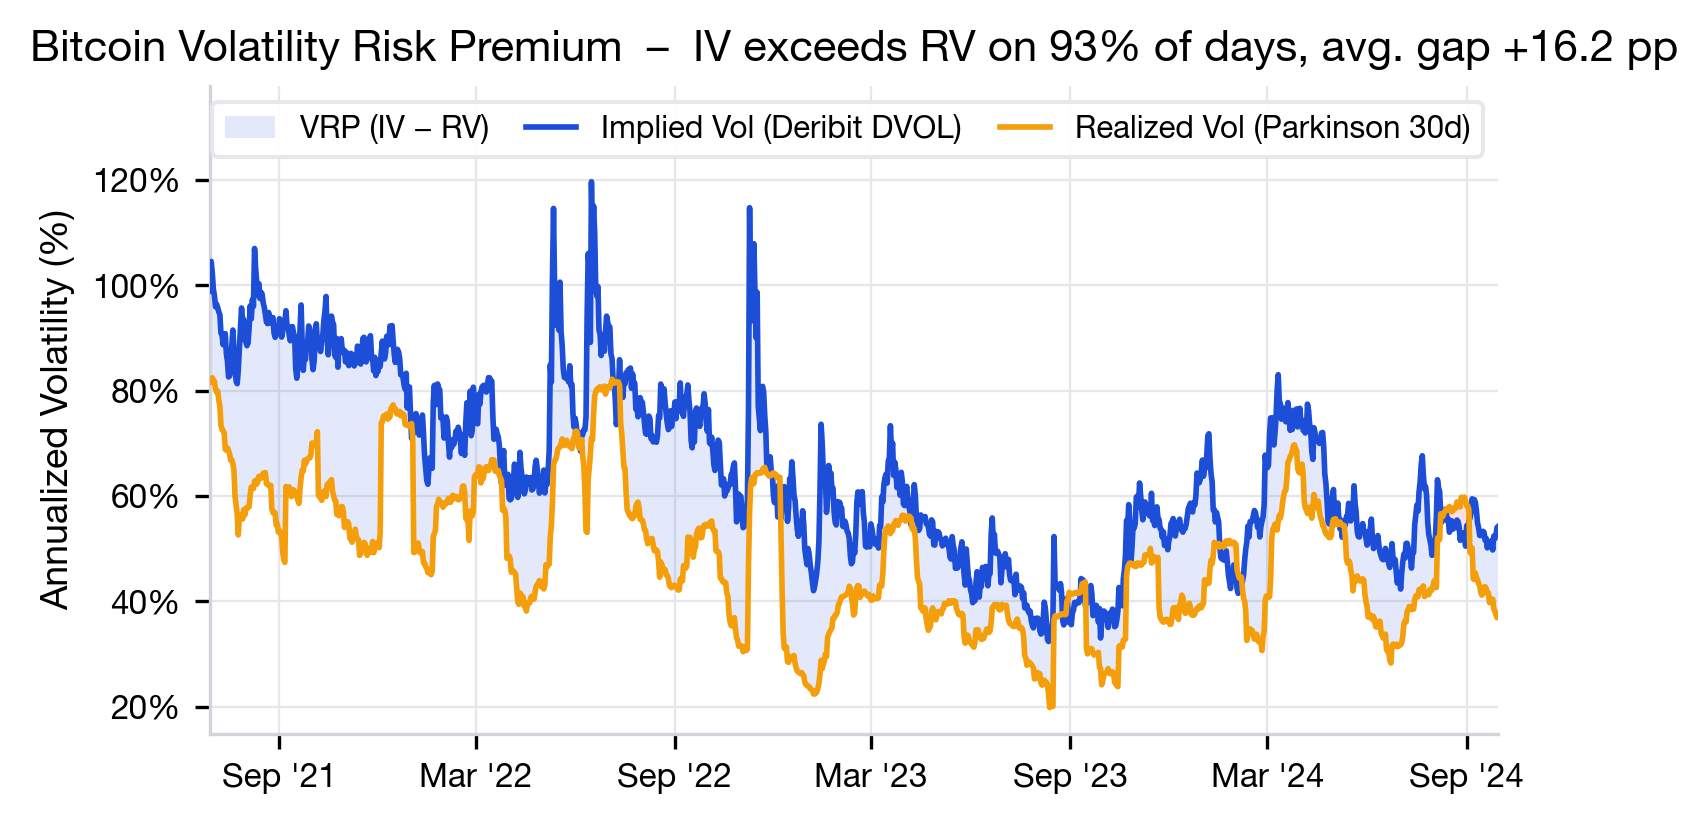
\includegraphics[width=\textwidth]{figures/fig1_vrp.png}
\caption{Volatilità implicita (DVOL) e volatilità realizzata a 30 giorni
(Parkinson) su Bitcoin, giugno 2021 -- settembre 2024. Lo spread medio di
16,2 punti percentuali costituisce il premio per il rischio di volatilità
oggetto di questa tesi.}
\label{fig:vrp-btc}
\end{figure}

Le ragioni strutturali di un VRP così ampio sul mercato crypto sono
riconducibili alla composizione dei flussi: la domanda di opzioni è
dominata dal lato acquisti: investitori retail che comprano call a leva
e operatori nativi del settore (miner, società con tesorerie in Bitcoin)
che comprano put a copertura, mentre l'offerta di volatilità è limitata
dalla scarsità di market maker con capitale dedicato. Il risultato è un
mercato strutturalmente \emph{long gamma} dal lato della domanda, in cui
chi vende volatilità viene remunerato con un premio persistente.

\section{Domanda di ricerca}
\label{sec:intro-research-question}

La domanda di ricerca di questa tesi è la seguente: \emph{il premio per il
rischio di volatilità sulle opzioni Bitcoin è catturabile in modo
sistematico, al netto di costi di transazione realistici, attraverso una
strategia replicabile di vendita di opzioni con copertura delta?}

La risposta richiede di affrontare tre problemi distinti:

\begin{enumerate}
\item \textbf{Selezione}: quale opzione vendere, ogni giorno, tra le
centinaia quotate? Esiste un segnale che discrimini i momenti e gli
strumenti migliori, o la scelta più semplice è anche la migliore?
\item \textbf{Esecuzione e copertura}: come neutralizzare l'esposizione
direzionale al sottostante, e con quale strumento (futures perpetui o
trimestrali), tenendo conto dei costi di ribilanciamento?
\item \textbf{Dimensionamento}: quanta esposizione assumere per trade, in
funzione del capitale, in modo da rendere sostenibili i drawdown di una
strategia short volatility priva di stop loss?
\end{enumerate}

\section{Contributi e metodo}
\label{sec:intro-contributi}

Il contributo di questa tesi non risiede in un modello complesso, ma nel
rigore del processo di eliminazione che conduce alla strategia finale.
Cinque ipotesi progressivamente più sofisticate sono state costruite,
testate e scartate con criteri statistici espliciti:

\begin{enumerate}
\item lo scoring basato sul gap tra densità risk-neutral e densità fisica
(nessun potere predittivo: $\beta < 0$, $p = 0{,}37$);
\item la selezione Premium/DTE (la redditività apparente era interamente
un artefatto dei dati: il 116\% dei profitti proveniva da opzioni illiquide
con bid nullo all'uscita);
\item la modalità multi-posizione (drawdown in-sample del $-49{,}7\%$
durante il crash del 2022);
\item cinque filtri di regime (nessuna correlazione con il PnL per trade
superiore a 0,25 in valore assoluto);
\item lo stop loss (a ogni soglia testata distrugge più profitto dai
trade vincenti di quanto ne salvi dai perdenti).
\end{enumerate}

La strategia sopravvissuta a questo processo è la più semplice possibile:
vendere ogni giorno l'opzione con il vega più alto nell'universo filtrato
($|\Delta| \le 0{,}50$), coprire il delta con futures trimestrali, uscire
al 50\% del premio incassato o a 5 giorni dalla scadenza. Su 35 trade
in-sample (giugno 2021 -- settembre 2023, periodo che include il bear
market del 2022 con un trimestre a $-55\%$ per Bitcoin) la strategia
produce uno Sharpe ratio di 1,75, statisticamente significativo all'1\%
($p = 0{,}007$). Out-of-sample (ottobre 2023 -- settembre 2024) lo Sharpe è
1,52.

Tre elementi rafforzano la credibilità del risultato. Primo, un audit
sistematico del backtest ha identificato e corretto distorsioni che
gonfiavano i risultati preliminari (uscite valorizzate al bid anziché
all'ask, costi di transazione assenti, opzioni illiquide con prezzi
fittizi). Secondo, la validazione cross-asset: la stessa strategia,
applicata senza alcuna riottimizzazione alle opzioni SPY su 14 anni di dati
(147 trade), produce un win rate della gamba opzionaria identico (82\%),
confermando che il meccanismo di cattura del VRP non è un artefatto del
campione Bitcoin. Terzo, l'implementazione live: la strategia è operativa
in paper trading sulla testnet di Deribit, con esecuzione automatizzata
ogni quattro ore, a verifica della replicabilità operativa dell'intera
pipeline.

\section{Struttura della tesi}
\label{sec:intro-struttura}

Il Capitolo~\ref{ch:letteratura} colloca il lavoro nella letteratura sul
VRP e sui mercati delle opzioni crypto. Il
Capitolo~\ref{ch:dati} descrive i dati, il mercato Deribit e
l'infrastruttura di backtest, inclusa l'estrazione della densità
risk-neutral e la costruzione del framework walk-forward. Il
Capitolo~\ref{ch:percorso} documenta il percorso di ricerca: le cinque
ipotesi testate e scartate. Il Capitolo~\ref{ch:strategia} presenta la
strategia finale Top Vega. Il Capitolo~\ref{ch:money-management} sviluppa
il money management: dimensionamento capital-based, sanity check di Kelly,
margini e simulazione Monte Carlo del rischio di rovina. Il
Capitolo~\ref{ch:validazione} contiene la validazione statistica e
cross-asset. Il Capitolo~\ref{ch:paper-trading} descrive l'implementazione
live. Il Capitolo~\ref{ch:limitazioni} discute le limitazioni e gli
sviluppi futuri. Il Capitolo~\ref{ch:conclusioni} conclude.

\chapter{Rassegna della letteratura}
\label{ch:letteratura}

Questo capitolo colloca il lavoro all'interno di cinque filoni di ricerca.
Il primo definisce il premio per il rischio di volatilità nei mercati
tradizionali e ne discute le spiegazioni teoriche
(\S\ref{sec:lit-vrp-tradizionale}). Il secondo esamina le strategie
sistematiche di vendita di volatilità e il loro profilo di rischio
(\S\ref{sec:lit-short-vol}). Il terzo passa al mercato delle opzioni su
criptovalute, dove il fenomeno assume dimensioni particolari
(\S\ref{sec:lit-crypto-options}). Il quarto e il quinto trattano gli
strumenti metodologici impiegati nella tesi: la stima della volatilità
realizzata (\S\ref{sec:lit-realized-vol}) e l'estrazione della densità
risk-neutral (\S\ref{sec:lit-rnd}), oltre ai criteri di dimensionamento del
rischio (\S\ref{sec:lit-sizing}). Il capitolo si chiude posizionando il
contributo di questa tesi (\S\ref{sec:lit-posizionamento}).

\section{Il Volatility Risk Premium nei mercati tradizionali}
\label{sec:lit-vrp-tradizionale}

Il premio per il rischio di volatilità (VRP) è la differenza sistematica
tra la volatilità implicita nei prezzi delle opzioni e la volatilità che il
sottostante realizza successivamente. Empiricamente questa differenza è
positiva e persistente: chi vende opzioni, e dunque vende volatilità,
incassa in media un premio, mentre chi le acquista paga un costo atteso
superiore al valore attuariale della protezione ottenuta.

La prima evidenza sistematica del fenomeno su singole azioni e indici si
deve a \citet{bakshi2003delta}, che studiano i rendimenti di posizioni in
opzioni coperte in delta (\emph{delta-hedged gains}). Se il modello di
Black--Scholes valesse esattamente e non esistesse alcun premio per il
rischio di volatilità, il guadagno di una posizione coperta in delta
dovrebbe essere nullo in media. Gli autori documentano invece guadagni
sistematicamente negativi per chi detiene le opzioni, e li interpretano
come prezzo di mercato di un rischio di volatilità priced negativamente:
gli investitori sono disposti a pagare per detenere strumenti che
guadagnano quando la volatilità sale.

\citet{carr2009variance} formalizzano il concetto attraverso i
\emph{variance swap}, la cui gamba fissa (il tasso di variance swap) è
replicabile in modo model-free da un portafoglio statico di opzioni su un
continuum di strike. La differenza tra il tasso di variance swap
(volatilità attesa sotto la misura risk-neutral $\mathbb{Q}$) e la varianza
effettivamente realizzata (sotto la misura fisica $\mathbb{P}$) misura
direttamente il variance risk premium. Su indici e single name statunitensi
il premio è ampiamente negativo per i compratori, coerentemente con
\citet{bakshi2003delta}.

\citet{bollerslev2009expected} mostrano che il VRP non è solo un premio
statico ma ha contenuto informativo: la differenza tra varianza implicita e
varianza realizzata prevede i rendimenti azionari futuri, con potere
predittivo particolarmente forte sull'orizzonte trimestrale. Gli autori
collegano il premio all'avversione al rischio aggregata e alla variabilità
temporale dell'incertezza economica, offrendo un fondamento di equilibrio
al fenomeno. Le principali spiegazioni teoriche del VRP, non
mutuamente esclusive, sono infatti tre: l'avversione degli investitori a
uno stato del mondo (alta volatilità) in cui la ricchezza marginale è
elevata; la domanda strutturale di copertura, che spinge i prezzi delle
opzioni sopra il loro valore attuariale; e i vincoli di capitale e di
inventario dei market maker, che richiedono un compenso per assorbire
l'offerta di rischio di volatilità.

\section{Strategie sistematiche di vendita di volatilità}
\label{sec:lit-short-vol}

Se il VRP è un premio persistente, la sua cattura sistematica è in linea di
principio possibile vendendo opzioni. La letteratura sulle strategie
passive di vendita di volatilità nasce con \citet{whaley2002return}, che
analizza l'indice CBOE S\&P~500 BuyWrite (BXM), una strategia
\emph{buy-write} che detiene l'indice e vende sistematicamente call
at-the-money. Whaley documenta, sul periodo 1988--2001, rendimenti
corretti per il rischio superiori a quelli del sottostante e, soprattutto,
una marcata riduzione della volatilità del portafoglio: la vendita
sistematica della call converte parte del premio per il rischio di
volatilità in reddito, al costo di rinunciare all'upside.

Questa letteratura evidenzia però anche il profilo di rischio asimmetrico
delle strategie short volatility. Il payoff tipico è composto da molti
piccoli guadagni intervallati da rare perdite di grande entità, un profilo
sintetizzato dalla metafora del \emph{picking up nickels in front of a
steamroller}. Tre implicazioni sono rilevanti per questa tesi. Primo, le
metriche basate sui soli momenti secondi (come lo Sharpe ratio) possono
sovrastimare la qualità di queste strategie, che concentrano il rischio
nelle code. Secondo, il dimensionamento della posizione e la gestione del
rischio di coda sono determinanti quanto la selezione dell'opzione. Terzo,
l'uso di stop loss su strategie short volatility è problematico, perché la
componente di theta decay che genera il profitto richiede tempo e viene
troncata da uscite premature, un punto che la presente tesi verifica
empiricamente nel Capitolo~\ref{ch:percorso}.

\section{Il mercato delle opzioni su criptovalute}
\label{sec:lit-crypto-options}

Il mercato delle opzioni su Bitcoin è giovane ma già oggetto di una
letteratura empirica in rapida crescita. La quasi totalità dell'attività si
concentra su Deribit, che controlla oltre l'80\% del volume globale di
opzioni crypto \citep{alexander2023inverse}. Una specificità tecnica del
mercato è che gli strumenti quotati sono \emph{inverse options}: premio e
regolamento sono denominati in Bitcoin, mentre lo strike è in dollari.
\citet{alexander2023inverse} mostrano che l'applicazione ingenua della
formula di Black--Scholes standard alle inverse options produce volatilità
implicite distorte, e che la volatilità implicita corretta per la struttura
inverse è quasi sempre superiore a quella ottenuta con la formula standard:
un dettaglio metodologico di cui la costruzione della volatility
surface deve tenere conto.

Il contributo più direttamente rilevante per questa tesi è quello di
\citet{alexander2020bitcoin}, che costruiscono un indice di volatilità
implicita per Bitcoin analogo al VIX, il precursore di quello che
Deribit avrebbe poi standardizzato nell'indice DVOL, a partire da oltre
sette milioni di prezzi di opzioni campionati ogni 15 minuti. Gli autori
documentano un premio per il rischio di varianza su Bitcoin
significativamente più ampio di quello dei mercati azionari. Studi
successivi ne quantificano la magnitudine: \citet{almeida2024risk} stimano
un variance risk premium annualizzato su Bitcoin compreso tra il 7\% e il
14\%, contro il 2\% circa dell'S\&P~500, un premio dunque di un ordine
di grandezza superiore. Un risultato particolarmente rilevante del loro
lavoro è che il VRP è \emph{più elevato nei regimi di bassa volatilità}
(0,10--0,17) che in quelli di alta volatilità (0,04--0,12), a indicare che
la preoccupazione degli investitori per il rischio di varianza non è
semplicemente proporzionale al livello corrente di volatilità.

Sul segno e sulla catturabilità del premio, \citet{winkel2023pricing}
stimano i pricing kernel impliciti nelle opzioni Deribit, ossia il rapporto
tra densità risk-neutral e densità fisica, e trovano che gli investitori
pagano un premio sostanziale per assicurarsi contro i movimenti di prezzo
di breve termine, premio decrescente con la scadenza. La letteratura
converge sul fatto che il premio per il rischio di volatilità osservato su
Deribit è negativo e significativo, cosicché le strategie di vendita di
volatilità sono attese generare performance corrette per il rischio
positive. È precisamente questa l'ipotesi che la presente tesi mette alla
prova in modo sistematico e con costi di transazione realistici.

\section{Stima della volatilità realizzata}
\label{sec:lit-realized-vol}

La misurazione della volatilità realizzata è centrale per quantificare il
VRP, poiché costituisce il termine di confronto della volatilità implicita.
Lo stimatore close-to-close, basato sui soli prezzi di chiusura, ignora
l'informazione contenuta nell'escursione infragiornaliera dei prezzi.
\citet{parkinson1980extreme} propone uno stimatore basato sul range
high--low che, sotto l'ipotesi di moto browniano senza drift, è circa
cinque volte più efficiente dello stimatore close-to-close. Per Bitcoin,
che è negoziato senza interruzione 24 ore su 24 e 7 giorni su 7, lo
stimatore di Parkinson è particolarmente appropriato: non esistono
discontinuità di chiusura e l'informazione infragiornaliera è pienamente
disponibile e continua. Per questa ragione la tesi adotta la volatilità
realizzata di Parkinson a 30 giorni come misura di riferimento.

Sul fronte del \emph{forecasting} della volatilità, non impiegato nella
strategia finale ma rilevante per gli sviluppi futuri, i due riferimenti
canonici sono il modello GARCH di \citet{bollerslev1986generalized}, che
cattura la persistenza (clustering) della volatilità condizionata, e il
modello HAR-RV di \citet{corsi2009simple}, che approssima la memoria lunga
della volatilità realizzata combinando componenti giornaliere, settimanali
e mensili. Entrambi sono discussi nel Capitolo~\ref{ch:limitazioni} come
possibili vie per riabilitare un segnale di \emph{timing} del premio.

\section{Estrazione della densità risk-neutral}
\label{sec:lit-rnd}

Il risultato fondamentale sull'estrazione della densità risk-neutral (RND)
implicita nei prezzi delle opzioni è quello di \citet{breeden1978prices}:
la densità risk-neutral del sottostante alla scadenza è proporzionale alla
derivata seconda del prezzo della call rispetto allo strike. In pratica,
disponendo di prezzi di opzioni su un insieme discreto di strike, la RND si
ottiene interpolando la superficie di volatilità implicita (tipicamente con
spline o parametrizzazioni tipo SVI), convertendo in prezzi di call
continui e differenziando numericamente due volte.

Questa infrastruttura è stata impiegata nella presente ricerca per
costruire un segnale di selezione delle opzioni, confrontando la RND (sotto
la misura $\mathbb{Q}$) con una stima della densità fisica (sotto la misura
$\mathbb{P}$) ottenuta via kernel density estimation. La letteratura
avverte tuttavia sulla fragilità del confronto \emph{pointwise} tra due
densità entrambe stimate con errore: la RND è sensibile agli errori di
interpolazione sulle code, e la densità fisica dipende in modo critico da
assunzioni di stazionarietà e dalla scelta della finestra. Come documentato
nel Capitolo~\ref{ch:percorso}, questa fragilità è la ragione empirica per
cui il segnale basato sul gap RND--KDE si è rivelato privo di potere
predittivo, pur restando la RND un utile strumento di contesto. La stessa
metodologia di stima dei pricing kernel è al centro del lavoro di
\citet{winkel2023pricing} e \citet{almeida2024risk} sul mercato Bitcoin.

\section{Criteri di dimensionamento e gestione del rischio}
\label{sec:lit-sizing}

Il problema del dimensionamento ottimo della posizione ha il suo
riferimento classico nel criterio di \citet{kelly1956new}, che massimizza
il tasso di crescita atteso del capitale nel lungo periodo. Il criterio di
Kelly è tuttavia noto per essere aggressivo e per essere estremamente
sensibile agli errori di stima dei parametri (probabilità di vincita e
rapporto payoff): quando questi sono stimati su campioni ridotti,
l'incertezza sulla frazione ottima è ampia e l'applicazione della frazione
piena espone a drawdown severi. La pratica di mercato adotta quindi
frazioni ridotte del Kelly (\emph{fractional Kelly}, tipicamente tra un
mezzo e un decimo), che sacrificano una piccola parte del tasso di crescita
atteso in cambio di una netta riduzione della variabilità del capitale.
Nella presente tesi il Half-Kelly è utilizzato non come metodo di
dimensionamento ma come \emph{sanity check} della ragionevolezza delle
configurazioni adottate (Capitolo~\ref{ch:money-management}), coerentemente
con l'osservazione che il vincolo operativo rilevante per una strategia
short volatility non è tanto il rischio di rovina quanto la tolleranza al
drawdown.

\section{Posizionamento di questa tesi}
\label{sec:lit-posizionamento}

Rispetto alla letteratura descritta, il contributo di questa tesi si
articola su tre piani. Primo, sul piano \emph{applicativo}: mentre gran
parte degli studi sul VRP crypto si concentra sulla misurazione del premio
(la sua esistenza, la sua magnitudine, il suo segno), questa tesi affronta
la domanda operativa di se e come il premio sia catturabile da una
strategia replicabile, al netto di costi di transazione realistici,
dell'esecuzione T+1 e della copertura delta. Secondo, sul piano
\emph{metodologico}: il lavoro documenta in modo trasparente non solo la
strategia sopravvissuta, ma anche le cinque ipotesi testate e scartate:
un antidoto al \emph{publication bias} che affligge la letteratura sulle
strategie di trading, dove tipicamente vengono riportati solo i risultati
positivi. In particolare, l'individuazione dell'artefatto da opzioni
illiquide con bid nullo (Capitolo~\ref{ch:percorso}) è un monito
metodologico di portata generale. Terzo, sul piano della \emph{robustezza}:
la validazione cross-asset su opzioni SPY, con la stessa strategia e senza
alcuna riottimizzazione, funge da test out-of-sample su una asset class
diversa e su un orizzonte temporale molto più lungo, isolando il meccanismo
di cattura del premio dalle specificità del campione Bitcoin.

\chapter{Dati e infrastruttura di ricerca}
\label{ch:dati}

Questo capitolo descrive il contesto istituzionale del mercato su cui opera
la strategia (\S\ref{sec:dati-deribit}), i dataset impiegati
(\S\ref{sec:dati-dataset}) e i tre pilastri metodologici dell'infrastruttura
di ricerca: la stima della volatilità realizzata
(\S\ref{sec:dati-rv}), l'estrazione della densità risk-neutral
(\S\ref{sec:dati-rnd}) e il framework di backtest walk-forward
(\S\ref{sec:dati-backtest}). Chiude con la caratterizzazione dei due periodi
di analisi (\S\ref{sec:dati-contesto}).

\section{Il mercato Deribit}
\label{sec:dati-deribit}

Deribit è la sede di negoziazione dominante per le opzioni su criptovalute,
con una quota superiore all'80\% del volume globale di opzioni Bitcoin. La
concentrazione della liquidità su un'unica piattaforma è una caratteristica
peculiare del mercato crypto e presenta un vantaggio per la ricerca: i
prezzi osservati provengono da un unico order book profondo, senza i
problemi di frammentazione e di consolidamento delle quotazioni tipici dei
mercati azionari multi-venue.

Le opzioni quotate su Deribit sono europee e di tipo \emph{inverse}: il
premio e il regolamento avvengono in Bitcoin, mentre lo strike è denominato
in dollari. Questa struttura ha un'implicazione tecnica rilevante per il
calcolo della volatilità implicita, poiché il payoff espresso in valuta di
base non è lineare nel prezzo del sottostante come nelle opzioni classiche.
La copertura direzionale della strategia utilizza i \emph{futures
trimestrali} anziché i \emph{perpetual}. La scelta è motivata dai costi: i
futures perpetui incorporano un tasso di \emph{funding} che, nei mercati
rialzisti, diventa strutturalmente oneroso per chi detiene posizioni corte,
mentre i futures trimestrali presentano una base fissa e prevedibile, priva
di funding. Deribit pubblica inoltre l'indice DVOL, una misura di
volatilità implicita a 30 giorni costruita con metodologia analoga al VIX,
che nel presente lavoro funge da riferimento per la volatilità implicita di
mercato.

\section{I dataset}
\label{sec:dati-dataset}

L'analisi si fonda su due corpora di dati principali: le opzioni Bitcoin di
Deribit per la strategia e per la validazione in-sample e out-of-sample, e
le opzioni SPY per la validazione cross-asset del
Capitolo~\ref{ch:validazione}. La Tabella~\ref{tab:dataset} ne riassume le
caratteristiche.

\begin{table}[H]
\centering
\caption{Dataset impiegati nell'analisi.}
\label{tab:dataset}
\small
\begin{tabular}{lllc}
\toprule
\textbf{Dato} & \textbf{Fonte} & \textbf{Frequenza} & \textbf{Periodo} \\
\midrule
Opzioni BTC (EOD) & Deribit & giornaliera & giu 2021 -- set 2024 \\
Spot BTC & Deribit & giornaliera & giu 2021 -- set 2024 \\
Perpetual BTC & Deribit & 5 minuti & giu 2021 -- set 2024 \\
Futures trimestrali BTC & Deribit & giornaliera (OHLC) & giu 2021 -- set 2024 \\
Funding rate & Deribit & giornaliera & giu 2021 -- set 2024 \\
Indice DVOL & Deribit & giornaliera & giu 2021 -- set 2024 \\
Opzioni SPY (EOD) & optionsDX & giornaliera & gen 2010 -- dic 2023 \\
\bottomrule
\end{tabular}
\end{table}

I file EOD mensili delle opzioni Bitcoin sono stati consolidati in un unico
dataset per il backtest. I prezzi delle opzioni sono espressi in Bitcoin
(coerentemente con la struttura inverse) e convertiti in dollari al prezzo
spot del giorno dove necessario per il calcolo del profitto e delle
metriche di rischio. Il dataset SPY, impiegato solo per la validazione
cross-asset, comprende file EOD giornalieri per quattordici anni, per un
totale di circa 9,5 milioni di record.

La qualità dei dati è un tema centrale per una strategia che vende opzioni,
poiché le distorsioni nei prezzi di strumenti illiquidi possono generare
profitti fittizi. Due aspetti meritano segnalazione. Primo, sul mercato
Bitcoin le opzioni profondamente in-the-money sono spesso prive di
quotazioni reali: il loro \emph{bid} nei dati risulta pari a zero, non
perché abbiano valore nullo ma perché nessun operatore le quota in
acquisto. Come documentato nel Capitolo~\ref{ch:percorso}, questo dettaglio
è all'origine di un artefatto che ha invalidato una delle strategie
esplorate, e ha motivato l'introduzione di un filtro sul delta. Secondo,
nel dataset SPY tre record su 9,5 milioni presentano volatilità implicita
negativa nei dati sorgente, con impatto trascurabile ($-11$ dollari sul
profitto totale) ma segnalato per completezza.

\section{Stima della volatilità realizzata}
\label{sec:dati-rv}

La quantificazione del premio per il rischio di volatilità richiede una
misura della volatilità effettivamente realizzata dal sottostante, da
confrontare con quella implicita nei prezzi delle opzioni. Come discusso
nel Capitolo~\ref{ch:letteratura}, la tesi adotta lo stimatore di
\citet{parkinson1980extreme}, basato sull'escursione infragiornaliera
high--low anziché sui soli prezzi di chiusura:
%
\begin{equation}
\hat{\sigma}^2_{P} = \frac{1}{4\ln 2}\,\frac{1}{n}\sum_{i=1}^{n}
\left(\ln \frac{H_i}{L_i}\right)^2,
\label{eq:parkinson}
\end{equation}
%
dove $H_i$ e $L_i$ sono rispettivamente il massimo e il minimo del giorno
$i$, e la stima viene annualizzata e calcolata su una finestra mobile di 30
giorni. La scelta è particolarmente appropriata per Bitcoin, negoziato
ininterrottamente 24 ore su 24 e 7 giorni su 7: l'assenza di sessioni di
chiusura elimina i salti overnight che affliggerebbero lo stimatore
close-to-close, e l'informazione contenuta nel range infragiornaliero è
pienamente disponibile e continua. Sotto le ipotesi del modello, lo
stimatore di Parkinson è circa cinque volte più efficiente di quello basato
sulle sole chiusure.

Il confronto tra il DVOL (volatilità implicita) e la volatilità realizzata
di Parkinson a 30 giorni, mostrato nella Figura~\ref{fig:vrp-btc} del
Capitolo~\ref{ch:introduzione}, evidenzia uno spread medio di 16,2 punti
percentuali annualizzati, positivo nel 93\% delle giornate. È questo il
premio che la strategia si propone di catturare.

\section{Estrazione della densità risk-neutral}
\label{sec:dati-rnd}

L'infrastruttura include una pipeline per l'estrazione della densità
risk-neutral (RND) implicita nei prezzi delle opzioni, basata sul risultato
di \citet{breeden1978prices}, secondo cui la RND è proporzionale alla
derivata seconda del prezzo della call rispetto allo strike:
%
\begin{equation}
q(K) = e^{rT}\,\frac{\partial^2 C(K,T)}{\partial K^2}.
\label{eq:breeden}
\end{equation}
%
In pratica, per ogni giornata e per ogni scadenza la pipeline procede in
quattro passi. Primo, costruisce la \emph{smile} di volatilità implicita a
partire dalle opzioni out-of-the-money (più liquide), applicando la
put-call parity per ricucire il ramo delle put con quello delle call.
Secondo, interpola la smile con una spline cubica su una griglia densa di
strike nell'intervallo di moneyness $[0{,}7;\,1{,}3]$. Terzo, converte le
volatilità interpolate in prezzi di call continui e vi adatta una spline di
quarto grado, di cui calcola analiticamente la derivata seconda per
ottenere la RND secondo l'Equazione~\eqref{eq:breeden}. Il tasso privo di
rischio è posto pari a zero, coerentemente con la prassi per gli strumenti
inverse denominati in Bitcoin. Quarto, la densità viene valutata su una
griglia di 200 punti e normalizzata.

Parallelamente, l'infrastruttura stima la densità fisica (sotto la misura
$\mathbb{P}$) tramite kernel density estimation gaussiana sui log-rendimenti
giornalieri, su una finestra mobile di 365 giorni, con bandwidth di
Silverman $h = 1{,}06\,\sigma\,N^{-1/5}$. Il confronto tra le due densità
era alla base di uno dei segnali di selezione esplorati. Come documentato
nel Capitolo~\ref{ch:percorso}, tale segnale si è rivelato privo di potere
predittivo, per ragioni riconducibili alla fragilità del confronto
\emph{pointwise} tra due densità entrambe stimate con errore; la RND resta
tuttavia un utile strumento di contesto e di analisi, e viene impiegata nel
Capitolo~\ref{ch:percorso} anche per il calcolo di skewness e curtosi
implicite tra gli indicatori di regime testati.

La Figura~\ref{fig:rnd-kde} mostra un esempio rappresentativo delle due
densità, estratte con la pipeline descritta per il 15 giugno 2022, nel pieno
del bear market, per la scadenza a 44 giorni: la densità risk-neutral è
spostata verso destra e più dispersa rispetto alla densità fisica stimata
sui rendimenti storici, coerentemente con una volatilità implicita superiore
a quella realizzata.

\begin{figure}[H]
\centering
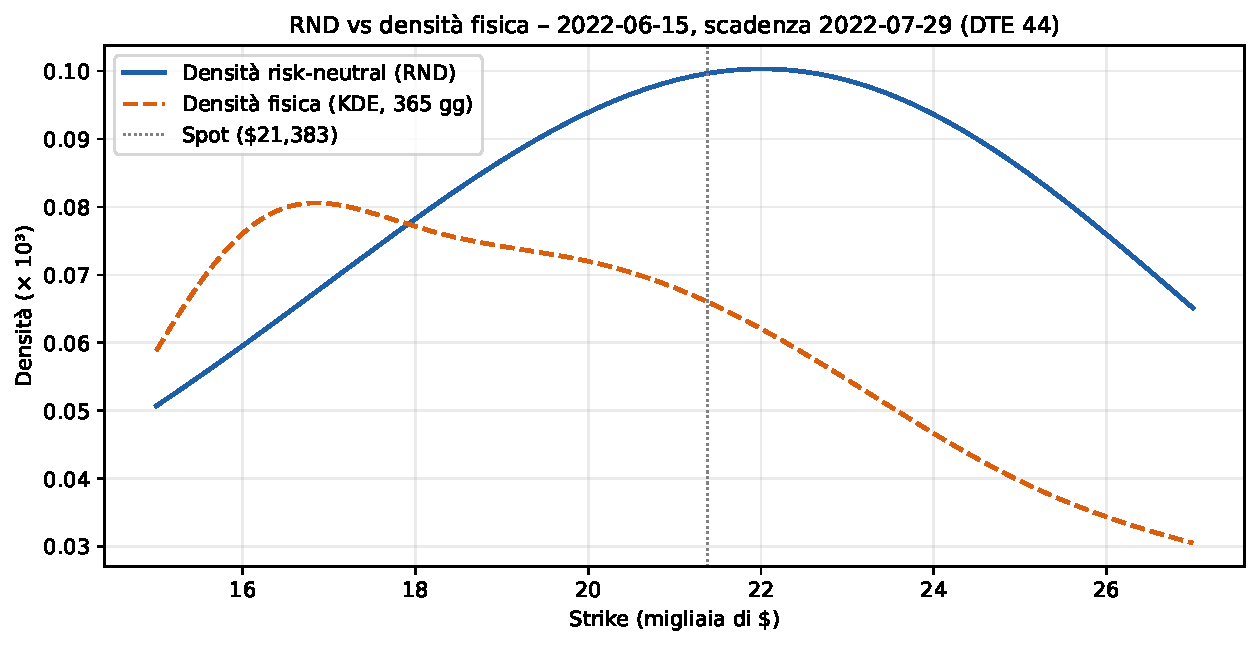
\includegraphics[width=\textwidth]{figures/fig_rnd_kde.pdf}
\caption{Densità risk-neutral (RND, estratta via Breeden--Litzenberger) e
densità fisica (KDE su 365 giorni di rendimenti) per il 15 giugno 2022,
scadenza 29 luglio 2022 (44 giorni). Spot: \$21.383.}
\label{fig:rnd-kde}
\end{figure}

\section{Il framework di backtest walk-forward}
\label{sec:dati-backtest}

Il backtest è organizzato in due fasi, separate per ragioni di efficienza
computazionale. La prima fase, di \emph{scoring}, percorre ogni giornata di
negoziazione, estrae la RND e la densità fisica, e assegna a ciascuna
opzione i punteggi previsti dalla strategia in esame; il suo output è un
file di punteggi precalcolati. La seconda fase, di \emph{simulazione},
legge i punteggi e replica l'attività di trading: selezione dell'opzione,
esecuzione, copertura delta giornaliera, applicazione delle regole di
uscita e imputazione dei costi. La separazione consente di eseguire una
sola volta la parte onerosa (l'estrazione delle densità) e di iterare
rapidamente sulle regole di simulazione.

Due scelte di disegno garantiscono l'assenza di look-ahead bias e il
realismo dei risultati. La prima è la \textbf{tempistica T+1}: il segnale è
calcolato sulla chiusura del giorno $T$, ma l'esecuzione avviene il giorno
$T+1$, al prezzo \emph{bid} dell'opzione (si vende) e al prezzo di apertura
del futures trimestrale. Nessuna informazione del giorno di esecuzione
entra nel segnale. La seconda è la \textbf{valorizzazione mark-to-market
giornaliera}: oltre al profitto realizzato a chiusura di ciascun trade,
l'infrastruttura ricostruisce la curva di equity giorno per giorno,
valorizzando la posizione aperta ai prezzi correnti. Il drawdown calcolato
sulla curva mark-to-market è molto più severo di quello calcolato sui soli
trade chiusi ed è la metrica di rischio primaria adottata in questa tesi,
perché riflette l'esperienza effettiva di chi detiene la posizione.

I costi di transazione sono modellati in modo granulare e conservativo, come
riassunto nella Tabella~\ref{tab:costi}. Le opzioni scontano la commissione
\emph{taker} di Deribit, pari allo 0,03\% del sottostante per lato, con il
tetto regolamentare del 12,5\% del prezzo dell'opzione; lo spread bid-ask è
incorporato direttamente valorizzando l'ingresso al bid e l'uscita all'ask.
La copertura sconta uno 0,10\% per lato, scomposto in commissione (0,05\%),
metà spread (0,03\%) e slippage (0,02\%).

\begin{table}[H]
\centering
\caption{Modello dei costi di transazione.}
\label{tab:costi}
\setlength{\tabcolsep}{4pt}
\begin{tabular}{lll}
\toprule
\textbf{Voce} & \textbf{Costo} & \textbf{Note} \\
\midrule
Commissione opzione & 0,03\% del sottostante / lato & cap al 12,5\% del premio \\
Spread opzione & incorporato & entry al bid, exit all'ask \\
Commissione hedge & 0,05\% / lato & futures trimestrali \\
Mezzo spread hedge & 0,03\% / lato & \\
Slippage hedge & 0,02\% / lato & \\
Funding & assente & scelta dei futures trimestrali \\
\bottomrule
\end{tabular}
\end{table}

L'analisi è condotta con una logica \emph{walk-forward}: i parametri e le
scelte di disegno sono fissati sul periodo in-sample e la loro tenuta è poi
verificata, senza alcuna riottimizzazione, sul periodo out-of-sample. Lo
split temporale, definito una volta per tutte, colloca l'in-sample dal
1\textsuperscript{o} giugno 2021 al 30 settembre 2023 e l'out-of-sample dal
1\textsuperscript{o} ottobre 2023 al 30 settembre 2024.

\section{Contesto di mercato dei due periodi}
\label{sec:dati-contesto}

La scelta dello split non è neutrale rispetto all'interpretazione dei
risultati, perché i due periodi presentano caratteristiche di mercato
profondamente diverse, riassunte nella Tabella~\ref{tab:contesto-mercato}.

\begin{table}[H]
\centering
\caption{Contesto di mercato dei periodi in-sample e out-of-sample.}
\label{tab:contesto-mercato}
\small
\setlength{\tabcolsep}{4pt}
\begin{tabular}{lcc}
\toprule
 & \textbf{In-sample} & \textbf{Out-of-sample} \\
 & giu 2021 -- set 2023 & ott 2023 -- set 2024 \\
\midrule
BTC inizio $\to$ fine & \$36.677 $\to$ \$26.916 ($-27\%$) & \$27.050 $\to$ \$64.543 ($+139\%$) \\
Range di prezzo & \$15.797 -- \$68.368 & \$26.777 -- \$73.285 \\
RV30 media & 57\% & 50\% \\
Carattere & Bear market + range & Bull market \\
 & (crash 2022: $-55\%$ in un trimestre) & (vol in compressione) \\
\bottomrule
\end{tabular}
\end{table}

Il periodo in-sample è il più severo e informativo: comprende il bear
market del 2022, con un trimestre a $-55\%$ per Bitcoin e le tensioni
seguite ai dissesti di operatori del settore. Una strategia short
volatility è strutturalmente esposta proprio agli episodi di questo tipo, in
cui la volatilità esplode e le posizioni corte in opzioni subiscono perdite
mark-to-market immediate. Che la strategia produca uno Sharpe elevato
attraversando questo periodo è dunque il risultato più solido dell'intero
lavoro. Il periodo out-of-sample, al contrario, è un mercato fortemente
rialzista con volatilità in compressione, un contesto favorevole alle
strategie di vendita di volatilità: il suo Sharpe, pur elevato, va letto
con la consapevolezza che le condizioni erano propizie, ed è
verosimilmente sovrastimato rispetto a un regime di mercato neutro. Questa
asimmetria interpretativa tra i due periodi guida la lettura dei risultati
nei capitoli successivi.

\chapter{Il percorso di ricerca: ipotesi testate e scartate}
\label{ch:percorso}

La strategia presentata in questa tesi è il risultato di un processo di
eliminazione. Prima di arrivare alla selezione Top Vega descritta nel
Capitolo~\ref{ch:strategia}, sono state costruite e testate cinque ipotesi
progressivamente più sofisticate, ciascuna scartata sulla base di un
criterio quantitativo esplicito. Documentare questo percorso, e non solo
l'esito, risponde a una precisa scelta metodologica: la letteratura sulle
strategie di trading è affetta da un marcato \emph{publication bias}, che
premia i risultati positivi e nasconde i tentativi falliti. Rendere
espliciti gli insuccessi ha due vantaggi. Da un lato, mostra che la
semplicità della strategia finale non è ingenuità ma il residuo di un
vaglio severo. Dall'altro, alcuni degli insuccessi (in particolare
l'artefatto documentato nella \S\ref{sec:percorso-premium-dte}) sono
lezioni metodologiche di portata generale per chiunque backtesti strategie
in opzioni su strumenti illiquidi.

\section{Ipotesi 1: il gap RND--KDE come segnale di selezione}
\label{sec:percorso-rnd-kde}

La prima ipotesi nasceva dall'idea più naturale in un contesto di vendita
di volatilità: se il premio esiste perché la densità risk-neutral
sovrastima la probabilità degli eventi estremi rispetto alla densità
fisica, allora il divario \emph{pointwise} tra le due densità dovrebbe
identificare le opzioni più sopravvalutate. Il punteggio assegnato a
ciascuna opzione era il prodotto tra il gap di probabilità (RND meno densità
fisica al relativo strike) e il vega dell'opzione, così da pesare il segnale
per la sensibilità alla volatilità. L'infrastruttura completa (segnale,
esecuzione, copertura, uscita, audit) è stata costruita con tempistica T+1 e
sottoposta a una griglia di sensibilità $6\times 5$, con celle tutte
profittevoli sia in-sample sia out-of-sample.

Il risultato apparentemente incoraggiante nascondeva però un problema di
fondo, emerso dal test critico. Non è sufficiente che il gap sia positivo
in media: il gap grezzo \emph{è} il premio per il rischio di volatilità, ed
è positivo quasi sempre proprio perché la volatilità implicita eccede
quella realizzata. Verificare che il gap grezzo sia positivo risponde alla
domanda banale, se il VRP esista, non alla domanda rilevante, se il segnale
sappia \emph{discriminare} i momenti e gli strumenti in cui vendere è più
conveniente. Per isolare la seconda domanda, il gap è stato reso a media
nulla (demeaned) tramite una media espansiva, strettamente causale, e
regredito sul profitto realizzato per trade con errori standard raggruppati
per data. Il coefficiente stimato è risultato negativo e non
significativo ($\beta < 0$, $p = 0{,}37$): il segnale, una volta rimossa la
componente banale, non ha alcun potere predittivo sul profitto dei singoli
trade. A conferma, un semplice benchmark che seleziona l'opzione a vega
massimo batteva la strategia complessa con meno trade e uno Sharpe
superiore.

La diagnosi è che il confronto pointwise tra due densità entrambe stimate
con errore produce un segnale dominato dal rumore. La densità fisica stimata
via kernel density estimation, sotto ipotesi di rendimenti indipendenti e
identicamente distribuiti su una finestra di 365 giorni, è troppo imprecisa
sulle code, proprio dove il gap dovrebbe essere informativo. Il gap è stato
dunque abbandonato come segnale di selezione, mentre la densità risk-neutral
è rimasta come infrastruttura tecnica e strumento di analisi.

\section{Ipotesi 2: la selezione Premium/DTE e l'artefatto bid=0}
\label{sec:percorso-premium-dte}

La seconda ipotesi puntava a massimizzare l'efficienza del premio per unità
di tempo, selezionando l'opzione con il rapporto più elevato tra premio
incassato e giorni alla scadenza (bid $\times$ spot / DTE). I risultati
iniziali erano notevoli: uno Sharpe in-sample di 1,67 su 126 trade, e una
correlazione quasi nulla con la selezione Top Vega, tale da suggerire un
portafoglio diversificato tra le due.

L'audit ha rivelato che l'intera redditività era un artefatto. Il problema
critico riguardava le opzioni profondamente in-the-money, che lo scoring
privilegiava perché caratterizzate da premi elevati (il delta mediano dei
trade selezionati era 0,99). Su Deribit queste opzioni sono di fatto
illiquide: nessun operatore le quota in acquisto, e il loro \emph{bid} nei
dati risulta pari a zero. Il backtest osservava quindi un prezzo di uscita
nullo, interpretava la posizione come chiusa avendo catturato il 100\% del
premio, e registrava un profitto inesistente. La
Tabella~\ref{tab:premium-dte-artefatto} scompone il fenomeno: 33 dei 126
trade (il 26\%) avevano prezzo di uscita nullo e generavano da soli 351.000
dollari, pari al 116,6\% del profitto totale di 301.000 dollari; i restanti
93 trade perdevano complessivamente 50.000 dollari. Senza l'artefatto, la
strategia era in perdita.

\begin{table}[H]
\centering
\caption{Scomposizione del profitto della strategia Premium/DTE (in-sample):
i trade con prezzo di uscita nullo, dovuti a opzioni illiquide, generano
oltre il 100\% dei profitti apparenti.}
\label{tab:premium-dte-artefatto}
\begin{tabular}{lcc}
\toprule
\textbf{Sottoinsieme di trade} & \textbf{Numero} & \textbf{Profitto aggregato} \\
\midrule
Trade con exit price $=0$ (illiquidi) & 33 & $+\$351.000$ \\
Trade con exit price $>0$ & 93 & $-\$50.000$ \\
\midrule
Totale apparente & 126 & $+\$301.000$ \\
\bottomrule
\end{tabular}
\end{table}

L'audit ha inoltre identificato due distorsioni minori ma sistematiche: le
uscite erano valorizzate al bid anziché all'ask (quando si riacquista
un'opzione corta si paga l'ask), e le opzioni non scontavano alcuna
commissione. Corretti tutti e tre i problemi (filtro sul delta $|\Delta| \le
0{,}50$ per escludere le opzioni deep in-the-money illiquide, uscita
all'ask, commissioni Deribit), lo Sharpe in-sample crollava a $-0{,}24$: la
strategia era morta.

Vale la pena notare che la prima interpretazione dell'anomalia era errata.
Si era ipotizzato che Premium/DTE fosse implicitamente una scommessa
direzionale, perché selezionava opzioni profondamente in-the-money. Ma se la
copertura delta funziona, anche un'opzione deep in-the-money è
delta-neutrale; il vero problema non era la direzionalità, bensì il prezzo
nullo nei dati. La diagnosi corretta è emersa solo scomponendo il profitto
dei singoli mega-trade, un promemoria del fatto che, nel backtesting di
strategie in opzioni, l'analisi aggregata può occultare artefatti che solo
l'ispezione trade per trade rivela.

\section{Ipotesi 3: multi-posizione per ampliare il campione}
\label{sec:percorso-multiposizione}

Una limitazione strutturale della strategia Top Vega è la bassa numerosità
campionaria: circa 35 trade in-sample in poco più di 800 giorni di
negoziazione. L'indagine ha mostrato che ciò non dipende da una scarsità di
segnali, ma dal lungo periodo di detenzione (DTE mediano all'ingresso di 66
giorni, holding medio di 25,5 giorni) combinato con il vincolo di posizione
singola: la strategia è di fatto investita per il 92,8\% del tempo (solo 61
giorni piatti su 851). Il problema non è la frequenza dei segnali, ma la
capacità di sfruttarli.

L'ipotesi naturale era allora consentire fino a tre posizioni simultanee,
diversificate per fascia di scadenza. La
Tabella~\ref{tab:multi-position} ne riporta i risultati.

\begin{table}[H]
\centering
\caption{Confronto tra posizione singola e multi-posizione (fino a 3
posizioni simultanee, diversificate per scadenza).}
\label{tab:multi-position}
\begin{tabular}{lcccc}
\toprule
\textbf{Metrica} & \textbf{Single IS} & \textbf{Multi IS} & \textbf{Single OOS} & \textbf{Multi OOS} \\
\midrule
Trade    & 35      & 147     & 10      & 60 \\
Sharpe   & 1,74    & 0,63    & 1,53    & 1,76 \\
Return   & 37\%    & 33\%    & 14\%    & 37\% \\
MTM DD   & $-18{,}4\%$ & $-49{,}7\%$ & $-4{,}5\%$ & $-14{,}5\%$ \\
\bottomrule
\end{tabular}
\end{table}

Il risultato è istruttivo perché la multi-posizione funziona nel periodo
out-of-sample (mercato calmo e rialzista) ma è devastante nel periodo
in-sample: il drawdown mark-to-market raggiunge il $-49{,}7\%$, contro il
$-18{,}4\%$ della posizione singola, con uno Sharpe che collassa da 1,74 a
0,63. La ragione è la correlazione: le posizioni parallele sono tutte corte
di volatilità sullo stesso sottostante, e durante un crash perdono
simultaneamente, mentre la copertura aggregata peggiora anziché migliorare.
La diversificazione per scadenza è illusoria quando il fattore di rischio
dominante, la volatilità di Bitcoin, è comune a tutte le posizioni. La
decisione è stata mantenere la posizione singola, accettando la bassa
frequenza come caratteristica intrinseca della strategia piuttosto che come
difetto da correggere.

\section{Filtri di regime: cinque indicatori senza potere predittivo}
\label{sec:percorso-regime}

L'analisi per regimi mostra che la strategia è forte in condizioni di
volatilità bassa e media e debole in alta volatilità, un profilo tipico
della vendita di volatilità. Ne discende l'ipotesi che un filtro capace di
ridurre l'esposizione, o di astenersi dal trading, nei momenti di alta
volatilità possa migliorare il rendimento corretto per il rischio. Per
verificarla, per ciascuno dei 35 trade in-sample è stato registrato il
valore di cinque indicatori al momento dell'ingresso, e ne è stata testata
la correlazione con il profitto del trade. La
Tabella~\ref{tab:regime-indicatori} riporta i risultati.

\begin{table}[H]
\centering
\caption{Indicatori di regime testati: correlazione con il profitto per
trade sui 35 trade in-sample. Nessun indicatore discrimina tra trade
vincenti e perdenti.}
\label{tab:regime-indicatori}
\begin{tabular}{lccc}
\toprule
\textbf{Indicatore} & \textbf{Corr. con PnL} & \textbf{Media winner} & \textbf{Media loser} \\
\midrule
DVOL (IV implicita)        & $+0{,}202$ & 76,4\%   & 74,6\% \\
Parkinson RV30             & $+0{,}237$ & 67,9\%   & 65,2\% \\
VRP spread (DVOL$-$RV30)   & $-0{,}133$ & 8,5 pp   & 9,4 pp \\
Skewness RND               & $-0{,}009$ & $-0{,}038$ & $-0{,}027$ \\
Curtosi RND                & $-0{,}086$ & 2,753    & 2,573 \\
\bottomrule
\end{tabular}
\end{table}

La scelta degli indicatori era economicamente motivata. Il DVOL misura il
livello della volatilità implicita, ossia quanto il mercato prezza la
volatilità futura; la RV30 di Parkinson misura il livello di volatilità
realizzata; lo spread tra i due è la misura più diretta del premio che si
sta vendendo, e concettualmente la più rilevante, perché se fosse invertito
(volatilità realizzata superiore all'implicita) non vi sarebbe premio da
catturare. La skewness e la curtosi della densità risk-neutral misurano
rispettivamente il rischio di coda e la pesantezza delle code prezzate dal
mercato.

Il risultato è che nessuno degli indicatori discrimina: tutte le
correlazioni sono in valore assoluto inferiori a 0,25, e le medie degli
indicatori nei trade vincenti e perdenti sono quasi indistinguibili.
Particolarmente istruttivo è il caso dello spread VRP, il candidato più
promettente in teoria: la sua correlazione con il profitto è addirittura di
segno negativo, e vi sono trade con spread molto elevato all'ingresso ($+12$
e $+31$ punti percentuali) che chiudono comunque in perdita. L'osservazione
di fondo è che il premio all'ingresso non è il fattore che determina il
profitto: quel che conta è ciò che accade \emph{durante} il trade, cioè se
sopraggiungano salti improvvisi o esplosioni di volatilità, eventi non
prevedibili dalle condizioni al momento dell'ingresso. Con soli 35 trade e
correlazioni tutte inferiori a 0,25, qualsiasi filtro costruito su questi
indicatori sarebbe privo di validità statistica. Nessun filtro di regime è
stato quindi implementato.

\section{Stop loss: un'analisi controfattuale}
\label{sec:percorso-stoploss}

L'ultima ipotesi riguardava lo stop loss. Una strategia short volatility
priva di stop è esposta, in linea di principio, a perdite di grande entità,
e la sua assenza richiede una giustificazione. L'analisi ha ricostruito, per
ciascuno dei 35 trade in-sample, il profitto mark-to-market non realizzato
giorno per giorno, registrando la perdita massima attraversata e
confrontandola con l'esito finale.

Tre osservazioni emergono. Primo, i trade vincenti attraversano
frequentemente drawdown significativi prima di recuperare: 15 dei 23
vincitori hanno registrato una perdita non realizzata inferiore a $-500$
dollari, e nel caso estremo un trade è sceso a $-17.386$ dollari (pari al
$-15{,}5\%$ del capitale) per poi chiudere a $+995$ dollari. Secondo, i
trade perdenti trascorrono molto più tempo in territorio negativo: in media
il 59\% dei giorni (15,1 giorni) contro il 29\% dei vincenti (6,2 giorni).
Terzo, sette trade erano in profitto oltre i 500 dollari prima di chiudere
in perdita, segno che il profit target non si è attivato in tempo.

Il test quantitativo, riportato nella Tabella~\ref{tab:stop-loss}, confronta
per ciascuna soglia di stop il profitto che sarebbe stato distrutto sui
trade vincenti stoppati prematuramente con quello che sarebbe stato
risparmiato sui trade perdenti.

\begin{table}[H]
\centering
\caption{Effetto controfattuale dello stop loss sui 35 trade in-sample. A
ogni soglia, il profitto distrutto sui trade vincenti supera quello
risparmiato sui perdenti.}
\label{tab:stop-loss}
\setlength{\tabcolsep}{6pt}
\begin{tabular}{lcccc}
\toprule
\textbf{Soglia} & \makecell{\textbf{Trade}\\\textbf{colpiti}} & \makecell{\textbf{di cui}\\\textbf{vincenti}} & \makecell{\textbf{PnL vincenti}\\\textbf{perso}} & \makecell{\textbf{PnL perdenti}\\\textbf{salvato}} \\
\midrule
$-1{,}0\%$ & 15 & 8 & \$23.380 & $-\$6.692$ \\
$-2{,}0\%$ & 5  & 3 & \$14.312 & $-\$2.928$ \\
$-3{,}0\%$ & 3  & 2 & \$8.619  & $-\$182$ \\
$-5{,}0\%$ & 2  & 2 & \$8.619  & \$0 \\
\bottomrule
\end{tabular}
\end{table}

\begin{figure}[H]
\centering
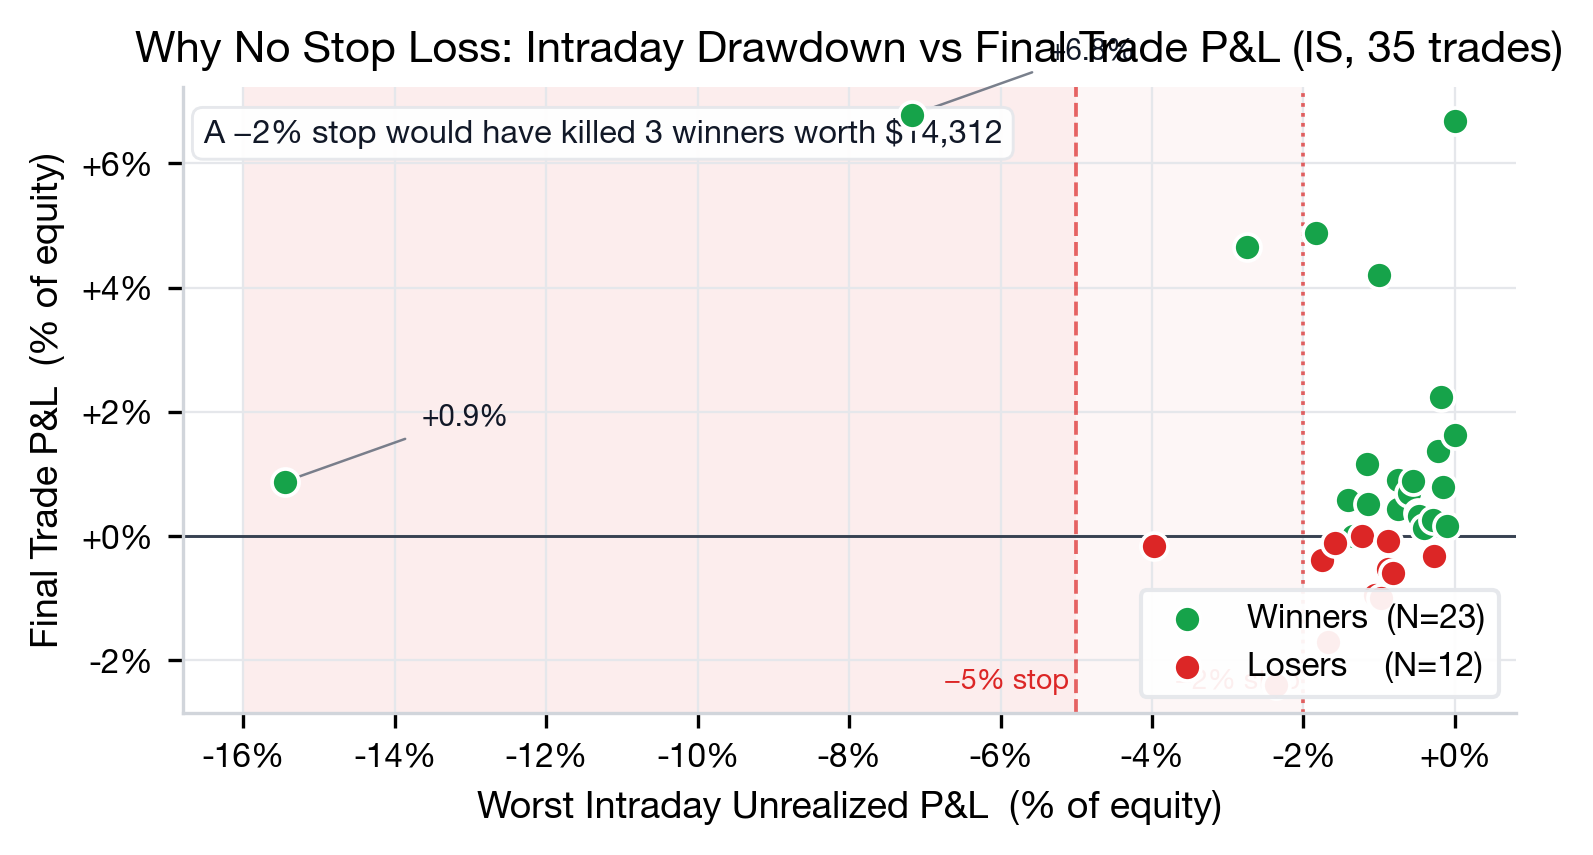
\includegraphics[width=\textwidth]{figures/fig3_stoploss.png}
\caption{Analisi dello stop loss: profitto distrutto sui trade vincenti
contro profitto risparmiato sui perdenti, per soglia di stop.}
\label{fig:stoploss}
\end{figure}

A ogni livello testato, il profitto perso sui vincenti stoppati supera
quello risparmiato sui perdenti; al di sotto del $-4\%$ verrebbero stoppati
soltanto trade vincenti. La spiegazione è economica: la strategia short
volatility genera profitto dal decadimento temporale (theta), che richiede
tempo per manifestarsi. Il profilo di payoff è asimmetrico nel tempo: la
perdita mark-to-market arriva subito, quando la volatilità implicita sale,
mentre il recupero è graduale e affidato al theta. Uno stop loss taglia
precisamente la fase di recupero, trasformando in perdite definitive
drawdown temporanei che si sarebbero riassorbiti. Nessuno stop loss è stato
quindi adottato: le uniche regole di uscita sono il profit target al 50\%
del premio e l'uscita temporale a 5 giorni dalla scadenza.

\section{Sintesi del processo di eliminazione}
\label{sec:percorso-sintesi}

La Tabella~\ref{tab:sintesi-decisioni} riepiloga le cinque ipotesi e il
criterio quantitativo che ha portato a scartarle. Il filo conduttore è che
ogni tentativo di aggiungere complessità, un segnale di selezione più
raffinato, un maggior numero di posizioni, un filtro di timing, una regola
di protezione, è stato sconfessato dai dati. La strategia sopravvissuta è la
più semplice tra quelle considerate, e la sua semplicità è il prodotto
diretto di questo vaglio, non una scelta di comodo.

\begin{table}[H]
\centering
\caption{Sintesi delle ipotesi testate e dei criteri di rigetto.}
\label{tab:sintesi-decisioni}
\small
\begin{tabular}{p{4.2cm}p{8.5cm}}
\toprule
\textbf{Ipotesi} & \textbf{Criterio di rigetto} \\
\midrule
Gap RND--KDE come segnale & $\beta < 0$, $p = 0{,}37$ sul gap demeaned regredito sul PnL; nessun potere predittivo \\
Selezione Premium/DTE & Il 116,6\% dei profitti era artefatto di prezzi di uscita nulli su opzioni illiquide; post-fix Sharpe $-0{,}24$ \\
Multi-posizione & Drawdown in-sample $-49{,}7\%$; le posizioni correlano nei crash \\
Filtri di regime & Cinque indicatori, tutte le correlazioni con il PnL inferiori a 0,25 \\
Stop loss & A ogni soglia distrugge più profitto sui vincenti di quanto ne salvi sui perdenti \\
\bottomrule
\end{tabular}
\end{table}

\chapter{La strategia finale: Top Vega}
\label{ch:strategia}

\section{Meccanismo economico}
\label{sec:strategia-meccanismo}

La strategia sopravvissuta al processo di eliminazione del
Capitolo~\ref{ch:percorso} è la più semplice tra quelle considerate: ogni
giorno seleziona e vende l'opzione con il vega più elevato nell'universo
filtrato. La motivazione economica è diretta. Il vega misura la sensibilità
del prezzo dell'opzione alla volatilità implicita; vendere l'opzione a vega
massimo significa massimizzare l'esposizione al premio per il rischio di
volatilità per unità di trade. Se il premio esiste, cioè se la volatilità
implicita eccede sistematicamente quella realizzata, allora concentrare
l'esposizione dove il vega è più alto è il modo più efficiente per
raccoglierlo. A differenza dei segnali esplorati nel
Capitolo~\ref{ch:percorso}, questa regola non contiene parametri da
stimare, non richiede il confronto tra densità e non pretende di prevedere
quando il premio sarà più ricco: si limita a raccoglierlo nel punto in cui
la sensibilità alla volatilità è massima.

Il profitto della strategia proviene da due fonti. La prima è la gamba
opzionaria: si incassa il premio e, se la volatilità realizzata resta
inferiore all'implicita prezzata, l'opzione decade a favore del venditore.
La seconda è la copertura delta: neutralizzando l'esposizione direzionale
con futures trimestrali e ribilanciando quotidianamente, la strategia
realizza un profitto dal ribilanciamento gamma quando il sottostante oscilla.
Come sarà quantificato nel Capitolo~\ref{ch:validazione}, su Bitcoin
l'81\% del profitto proviene dalla vendita di opzioni e il 19\% dalla
copertura: la strategia è dunque genuinamente una raccolta del premio di
volatilità, con la copertura che agisce da amplificatore su un sottostante
ad alta volatilità realizzata.

\section{Regole operative}
\label{sec:strategia-regole}

La Tabella~\ref{tab:configurazione} riassume la configurazione completa.

\begin{table}[H]
\centering
\caption{Configurazione completa della strategia Top Vega.}
\label{tab:configurazione}
\begin{tabular}{ll}
\toprule
\textbf{Componente} & \textbf{Regola} \\
\midrule
Selezione & opzione con $|\text{vega}|$ massimo, $|\Delta| \le 0{,}50$ \\
Posizioni & singola (max 1 aperta) \\
Entry & vendita al bid, esecuzione T+1 \\
Exit & riacquisto all'ask; profit target 50\% \emph{oppure} DTE $\le 5$ \\
Copertura & futures trimestrali Deribit, ribilanciamento giornaliero \\
Costi opzione & 0,03\% del sottostante per lato (cap Deribit) \\
Costi hedge & 0,10\% per lato (commissione, spread, slippage) \\
Stop loss & assente (controindicato, \S\ref{sec:percorso-stoploss}) \\
Filtri di regime & assenti (non predittivi, \S\ref{sec:percorso-regime}) \\
\bottomrule
\end{tabular}
\end{table}

Alcune scelte meritano una motivazione esplicita. Il filtro sul delta
($|\Delta| \le 0{,}50$) esclude le opzioni profondamente in-the-money, che
sul mercato Bitcoin sono illiquide e il cui prezzo nei dati è inaffidabile:
è la correzione che nel Capitolo~\ref{ch:percorso} ha smascherato
l'artefatto della strategia Premium/DTE. L'uscita a 5 giorni dalla scadenza
evita la zona in cui il gamma dell'opzione esplode e la copertura diventa
instabile e costosa. La scelta dei futures trimestrali per la copertura, in
luogo dei perpetui, elimina l'esposizione al tasso di funding, che nei
mercati rialzisti penalizza le posizioni corte. Il profit target al 50\% e
la soglia di uscita a 5 giorni sono parametri del backtest, non ottimizzati
sulla griglia di sensibilità: la robustezza della strategia alla loro
variazione è documentata nel Capitolo~\ref{ch:validazione}.

\section{Profilo dei trade selezionati}
\label{sec:strategia-profilo}

La regola Top Vega, pur non imponendo vincoli espliciti sulla scadenza o
sulla moneyness, seleziona in modo naturale un profilo di trade ben
definito, riassunto nella Tabella~\ref{tab:profilo-trade}. Poiché il vega di
un'opzione è massimo per strumenti vicini all'at-the-money e con scadenza
lontana, la strategia tende a vendere opzioni near-ATM (moneyness circa
1,04) con scadenza medio-lunga (DTE mediano all'ingresso di circa 66
giorni), mantenendole in media per 25 giorni. Questo profilo è coerente con
il meccanismo: sono proprio le opzioni ad alto vega quelle che offrono la
massima esposizione al premio di volatilità.

\begin{table}[H]
\centering
\caption{Profilo tipico dei trade selezionati dalla strategia Top Vega.}
\label{tab:profilo-trade}
\begin{tabular}{lc}
\toprule
\textbf{Metrica} & \textbf{Valore} \\
\midrule
DTE medio all'ingresso & $\sim$66 giorni \\
Moneyness & $\sim$1,04 (near-ATM) \\
IV media all'ingresso & $\sim$63\% \\
Holding period medio & $\sim$25 giorni \\
Vega per contratto & $\sim$49--98 \\
Meccanismo di profitto & raccolta del VRP (IV $>$ RV) \\
\bottomrule
\end{tabular}
\end{table}

\section{Risultati}
\label{sec:strategia-risultati}

La Tabella~\ref{tab:risultati-principali} riporta i risultati della
strategia nella configurazione di dimensionamento moderata (rischio 2\%,
buffer 1,5$\times$; il dimensionamento è trattato nel
Capitolo~\ref{ch:money-management}), su entrambi i periodi. Va sottolineato
fin d'ora che lo Sharpe ratio è invariante rispetto al dimensionamento,
poiché è un rapporto: le tre configurazioni di rischio scalano linearmente
rendimento e drawdown ma lasciano immutato lo Sharpe.

\begin{table}[H]
\centering
\caption{Risultati della strategia Top Vega, configurazione moderata
(rischio 2\%, buffer 1,5$\times$). Risultati post-audit.}
\label{tab:risultati-principali}
\begin{tabular}{lcc}
\toprule
\textbf{Metrica} & \textbf{In-sample} & \textbf{Out-of-sample} \\
\midrule
Trade & 35 & 10 \\
Sharpe ratio & 1,75 & 1,52 \\
Return & $+19{,}3\%$ & $+7{,}0\%$ \\
Max drawdown (MTM) & $-10{,}3\%$ & $-2{,}3\%$ \\
Win rate & 65,7\% & 70,0\% \\
t-test ($p$-value) & 0,007 & 0,091 \\
\bottomrule
\end{tabular}
\end{table}

\begin{figure}[H]
\centering
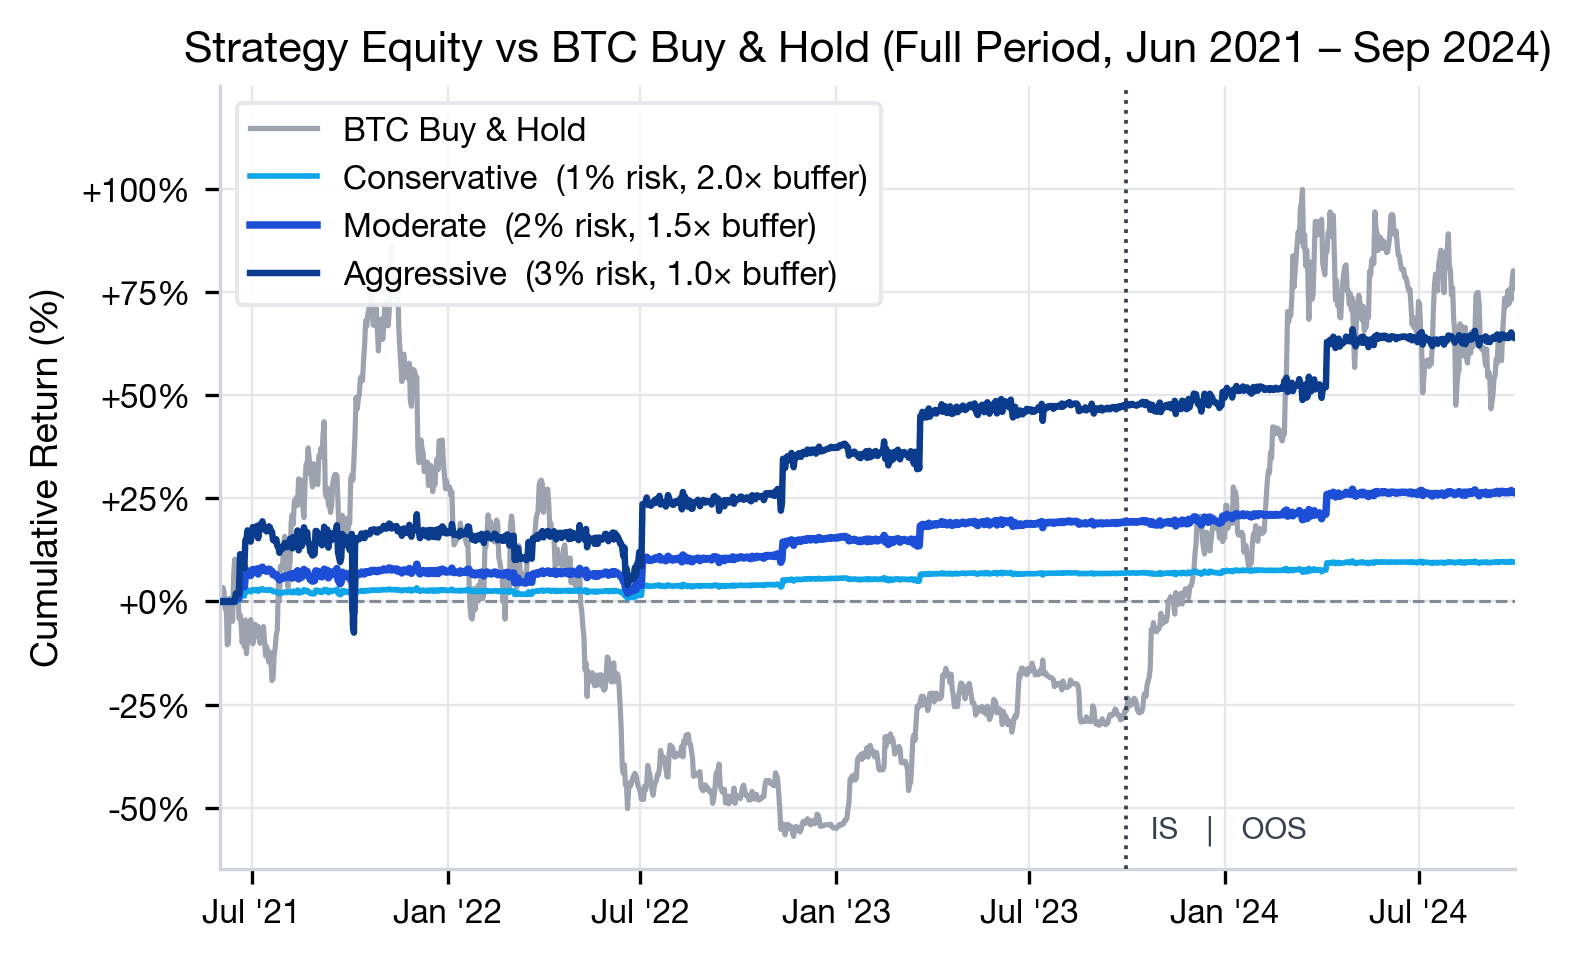
\includegraphics[width=\textwidth]{figures/fig2_equity.png}
\caption{Curva di equity mark-to-market della strategia Top Vega.}
\label{fig:equity}
\end{figure}

Il dato più solido è lo Sharpe in-sample di 1,75, ottenuto attraversando il
bear market del 2022 (Tabella~\ref{tab:contesto-mercato}). Come discusso nel
Capitolo~\ref{ch:dati}, l'in-sample è il periodo di prova più severo per una
strategia short volatility, proprio perché include l'episodio di stress cui
questa categoria di strategie è più esposta. Lo Sharpe out-of-sample, pari a
1,52, conferma la tenuta della strategia, ma va letto nel contesto di un
mercato rialzista con volatilità in compressione, favorevole alla vendita di
volatilità, e con soli 10 trade la sua stima è meno affidabile (il t-test
out-of-sample è significativo soltanto al 10\%). La validazione statistica
completa, comprensiva di intervalli di confidenza bootstrap e test di
robustezza, è sviluppata nel Capitolo~\ref{ch:validazione}.

Un'ultima osservazione riguarda la metrica di drawdown. I valori riportati
in tabella sono calcolati sulla curva mark-to-market, non sui soli trade
chiusi. Per una strategia che detiene posizioni in media per 25 giorni, il
drawdown mark-to-market è la misura onesta del rischio sopportato, perché
riflette le oscillazioni del valore della posizione lungo tutta la sua vita,
comprese le perdite non realizzate che, come mostrato
nella \S\ref{sec:percorso-stoploss}, i trade vincenti attraversano prima di
recuperare.

\chapter{Money management}
\label{ch:money-management}

\section{Evoluzione del dimensionamento}
\label{sec:mm-evoluzione}

Il dimensionamento della posizione è, per una strategia short volatility,
tanto importante quanto la selezione dell'opzione, perché determina
l'entità del rischio sopportato a parità di segnale. L'approccio adottato è
il risultato di una progressione in tre stadi. Il primo stadio, un contratto
fisso per trade, è problematico perché il rischio per trade oscilla con il
vega dell'opzione selezionata: due trade con lo stesso numero di contratti
possono comportare esposizioni alla volatilità molto diverse. Il secondo
stadio, un obiettivo di vega fisso (pari a 50), normalizza il rischio per
trade rendendolo indipendente dallo strumento, ma non si adatta al capitale:
dopo una serie di perdite o di guadagni, l'esposizione resta la stessa in
termini assoluti. Il terzo stadio, adottato nella tesi, lega l'obiettivo di
vega al capitale corrente.

La formula del dimensionamento \emph{capital-based} è la seguente:
%
\begin{equation}
\text{vega\_target} = \frac{\text{equity} \times \text{risk\_per\_trade}}
{\text{worst\_loss\_per\_vega} \times \text{buffer}},
\label{eq:sizing}
\end{equation}
%
dove \texttt{worst\_loss\_per\_vega} è calibrato sul peggior trade
in-sample (una perdita di 2.746 dollari su 50 vega, ossia 54,93 dollari di
perdita per unità di vega) e \texttt{buffer} è un moltiplicatore prudenziale
sul worst case. L'obiettivo di vega si ricalcola a ogni trade: cresce con il
capitale, realizzando il compounding, e si riduce dopo le perdite,
attenuando automaticamente l'esposizione nei drawdown.

Un aspetto metodologico va chiarito. Le diverse configurazioni di
dimensionamento sono ottenute per riscalatura a posteriori: i trade
selezionati (date di ingresso e di uscita, strumenti) sono identici in tutte
le configurazioni, e cambia soltanto la dimensione in dollari della
posizione. Ne consegue che lo Sharpe ratio è invariante rispetto alla
configurazione, essendo un rapporto tra rendimento medio e deviazione
standard: il dimensionamento sposta la scala di rendimento e drawdown, non
la loro proporzione.

\section{Le tre configurazioni di rischio}
\label{sec:mm-configurazioni}

La Tabella~\ref{tab:configurazioni-rischio} presenta tre configurazioni,
corrispondenti a diversi appetiti per il rischio. Il parametro
\texttt{risk\_per\_trade} passa dall'1\% al 3\% del capitale, mentre il
buffer prudenziale si riduce da 2,0 a 1,0, cosicché la configurazione
conservativa è doppiamente cauta (meno rischio per trade e buffer maggiore)
e quella aggressiva doppiamente incisiva.

\begin{table}[H]
\centering
\caption{Le tre configurazioni di rischio. Lo Sharpe ratio è invariante
rispetto al dimensionamento; il trade-off è esclusivamente tra rendimento e
drawdown.}
\label{tab:configurazioni-rischio}
\small
\setlength{\tabcolsep}{4pt}
\begin{tabular}{lcccccccc}
\toprule
\textbf{Config.} & \textbf{Risk} & \textbf{Buffer} & \makecell{\textbf{Vega}\\\textbf{in.}} & \textbf{Ret IS} & \textbf{DD IS} & \makecell{\textbf{Ret}\\\textbf{OOS}} & \makecell{\textbf{DD}\\\textbf{OOS}} & \makecell{\textbf{Sharpe}\\\textbf{IS/OOS}} \\
\midrule
Conservativa & 1\% & 2,0$\times$ & 9,1  & $+6{,}9\%$  & $-3{,}9\%$  & $+2{,}6\%$  & $-0{,}9\%$ & 1,75/1,52 \\
Moderata     & 2\% & 1,5$\times$ & 24,3 & $+19{,}3\%$ & $-10{,}3\%$ & $+7{,}0\%$  & $-2{,}3\%$ & 1,75/1,52 \\
Aggressiva   & 3\% & 1,0$\times$ & 54,6 & $+47{,}8\%$ & $-22{,}6\%$ & $+16{,}1\%$ & $-5{,}1\%$ & 1,75/1,52 \\
\bottomrule
\end{tabular}
\end{table}

L'invarianza dello Sharpe ha un'implicazione importante: la scelta della
configurazione non è una scelta di qualità della strategia, ma di
tolleranza al drawdown. Un investitore che accetti un drawdown atteso fino
al $-22{,}6\%$ in-sample può adottare la configurazione aggressiva e mirare
a un rendimento del $+47{,}8\%$; uno più prudente si accontenterà del
$+6{,}9\%$ della configurazione conservativa con un drawdown contenuto entro
il $-3{,}9\%$. La strategia sottostante è la medesima. La configurazione
aggressiva, con vega iniziale di 54,6, è peraltro quasi identica al vega
fisso pari a 50 dello stadio precedente: il vantaggio del dimensionamento
capital-based non è un'esposizione diversa, ma la sua adattività automatica
al capitale.

Non sono stati adottati altri metodi di dimensionamento per ragioni
specifiche. Il criterio di Kelly pieno, come discusso nella sezione
seguente, richiede stime di parametri troppo rumorose su 35 trade. Il
\emph{vol targeting} ha senso per portafogli multi-posizione con
correlazioni variabili, non per una strategia a posizione singola. Lo
\emph{scaling} sul drawdown è già incorporato implicitamente nel
dimensionamento capital-based, poiché un calo del capitale riduce
automaticamente l'obiettivo di vega.

\section{Half-Kelly come sanity check}
\label{sec:mm-kelly}

Il criterio di \citet{kelly1956new} è stato calcolato non come metodo di
dimensionamento, ma come verifica di coerenza della prudenza delle
configurazioni adottate. A partire dai 35 trade in-sample, con un win rate
del 65,7\% e un rapporto di payoff di 2,57 (guadagno medio 1,76\% contro
perdita media 0,69\%), la frazione di Kelly risulta
%
\begin{equation}
f^{*} = 0{,}657 - \frac{1 - 0{,}657}{2{,}57} = 52{,}4\%,
\end{equation}
%
e la sua metà (Half-Kelly), la frazione prudenziale di uso comune, vale il
26,2\%, corrispondente a un obiettivo di vega di circa 477. Il confronto con
le tre configurazioni è netto: la conservativa impiega il 2\% del
Half-Kelly, la moderata il 5\% e l'aggressiva l'11\%. Anche la
configurazione più incisiva opera dunque a poco più di un decimo del
Half-Kelly.

Questa estrema prudenza è intenzionale e proporzionata all'incertezza.
Trentacinque trade sono pochi per stimare con precisione i parametri di
Kelly, la cui sensibilità agli errori di input è nota. Il criterio assume
inoltre distribuzioni stazionarie e indipendenza tra i trade, ipotesi
fragili per una strategia esposta a salti e a esplosioni di volatilità, come
mostra il worst case in-sample (una perdita non realizzata del $-15{,}5\%$).
Nella prassi, del resto, nessun operatore istituzionale opera oltre il
10--15\% del Kelly. Il sanity check conferma quindi che le configurazioni
non sono irragionevolmente conservative, ma prudenti in misura commisurata
all'incertezza dei parametri.

\section{Margini Deribit e soglia di rovina}
\label{sec:mm-margini}

Il dimensionamento deve tenere conto dei margini richiesti dall'exchange. La
Tabella~\ref{tab:margini} riporta il margine iniziale, calcolato secondo la
formula Standard Margin di Deribit per opzioni corte, sui 35 trade
in-sample e per ciascuna configurazione.

\begin{table}[H]
\centering
\caption{Margine iniziale (Standard Margin Deribit) calcolato sui 35 trade
in-sample, per configurazione.}
\label{tab:margini}
\begin{tabular}{lccc}
\toprule
\textbf{Configurazione} & \textbf{IM medio} & \textbf{IM worst-case} & \textbf{Capitale min (1,5$\times$)} \\
\midrule
Conservativa (vega 9,1)  & \$1.672  & \$6.205  & \$9.308 \\
Moderata (vega 24,3)     & \$4.465  & \$16.570 & \$24.855 \\
Aggressiva (vega 54,6)   & \$10.033 & \$37.232 & \$55.847 \\
\bottomrule
\end{tabular}
\end{table}

Ne discende una soglia di rovina operativa di circa 10.000 dollari: al di
sotto di questo livello non è possibile aprire neppure un singolo trade
nella configurazione più conservativa mantenendo un buffer di margine
adeguato. Con il dimensionamento capital-based questa soglia vale per tutte
le configurazioni, poiché l'esposizione si adatta automaticamente al
capitale disponibile. Va notato che il margine worst-case include un trade
con delta pari a 0,75 all'ingresso: il filtro $|\Delta| \le 0{,}50$ è
applicato alla data del segnale, ma il delta si muove tra segnale ed
esecuzione (il trade in questione aveva delta $-0{,}495$ al segnale e
$-0{,}755$ all'ingresso, per effetto di un movimento overnight di Bitcoin).
Si tratta di uno scivolamento realistico e non evitabile.

\section{Rischio di rovina: simulazione Monte Carlo}
\label{sec:mm-montecarlo}

Il drawdown realizzato nel backtest è una singola traiettoria: per valutare
il rischio in modo prospettico occorre chiedersi quanto avrebbe potuto
essere diverso, a parità di caratteristiche statistiche della strategia. A
questo scopo è stata condotta una simulazione Monte Carlo basata sul
\emph{circular block bootstrap} dei rendimenti giornalieri mark-to-market
del periodo in-sample: per ciascuna configurazione, 10.000 percorsi della
stessa lunghezza del periodo in-sample (845 giorni) sono generati
ricampionando blocchi contigui di 20 giorni di rendimenti effettivi. Il
ricampionamento a blocchi, anziché per singole osservazioni, preserva il
raggruppamento temporale delle perdite (i giorni negativi tendono a
concentrarsi nei periodi di stress, come il crash del 2022), che è la
caratteristica che rende profondi i drawdown; i risultati sono robusti alla
scelta della lunghezza del blocco (la mediana varia di meno di un punto
percentuale tra blocchi di 5 e di 40 giorni). Accanto allo scenario base è
stato simulato uno scenario di stress dichiarato, in cui ogni rendimento
giornaliero negativo è amplificato del 50\% prima del ricampionamento: uno
scenario severo per costruzione, poiché il peggioramento si applica
sistematicamente per l'intero orizzonte. La soglia di rovina è fissata a
10.000 dollari (\S\ref{sec:mm-margini}).

\begin{table}[H]
\centering
\caption{Distribuzione del max drawdown dalla simulazione Monte Carlo
(block bootstrap dei rendimenti giornalieri MTM in-sample, 10.000 percorsi
di 845 giorni). La colonna ``realizzato'' riporta il drawdown
effettivamente osservato nel backtest: la sua vicinanza alla mediana
simulata conferma la coerenza del modello. P(rovina): frazione di percorsi
che raggiunge la soglia di 10.000 dollari.}
\label{tab:montecarlo-dd}
\footnotesize
\setlength{\tabcolsep}{3pt}
\begin{tabular}{lccccccc}
\toprule
 & & \multicolumn{3}{c}{\textbf{Scenario base}} & \multicolumn{2}{c}{\textbf{Stress ($\times$1,5)}} & \\
\cmidrule(lr){3-5}\cmidrule(lr){6-7}
\textbf{Configurazione} & \textbf{Realizz.} & \textbf{Mediana} & \textbf{P95} & \textbf{P99} & \textbf{Mediana} & \textbf{P95} & \textbf{P(rovina)} \\
\midrule
Conservativa (1\%) & $-3{,}9\%$  & $-3{,}7\%$  & $-5{,}9\%$  & $-7{,}5\%$  & $-18{,}0\%$ & $-25{,}0\%$ & 0{,}00\% \\
Moderata (2\%)     & $-10{,}3\%$ & $-9{,}7\%$  & $-15{,}1\%$ & $-18{,}8\%$ & $-41{,}6\%$ & $-54{,}6\%$ & 0{,}00\% \\
Aggressiva (3\%)   & $-22{,}6\%$ & $-21{,}4\%$ & $-31{,}9\%$ & $-38{,}7\%$ & $-71{,}4\%$ & $-83{,}9\%$ & 0{,}00\% \\
\bottomrule
\end{tabular}
\end{table}

\begin{figure}[H]
\centering
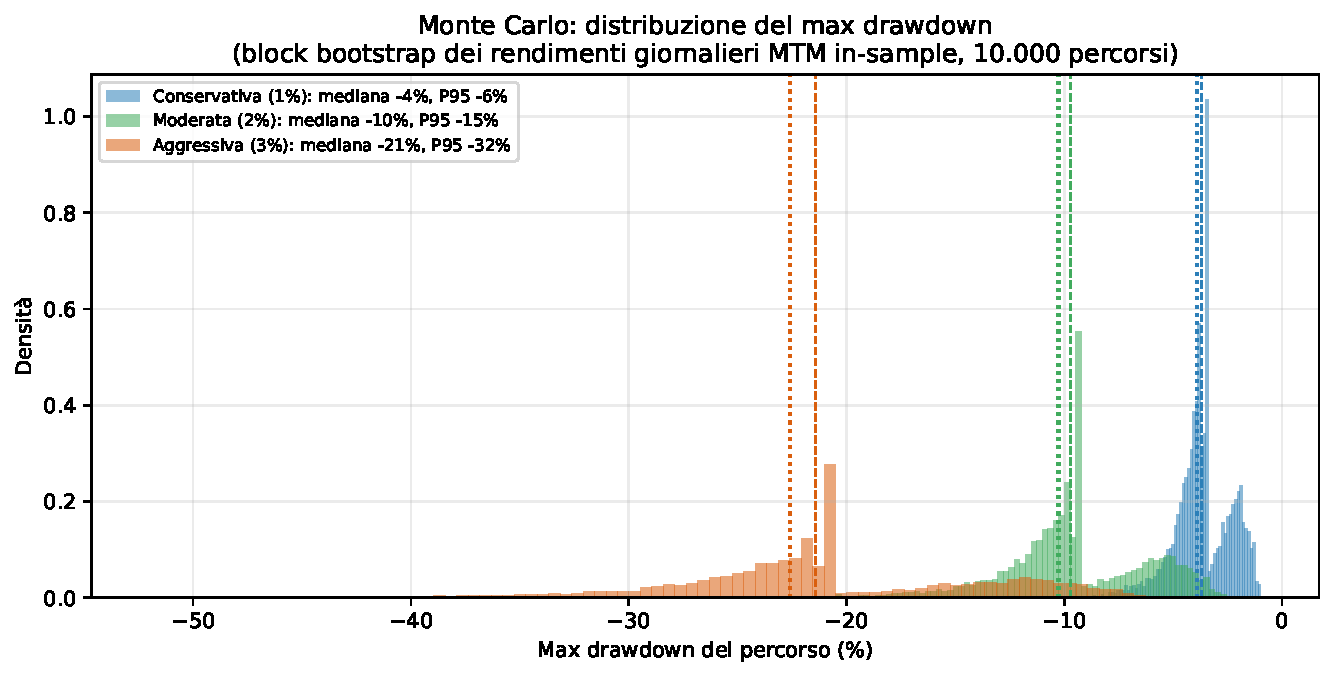
\includegraphics[width=\textwidth]{figures/fig_mc_drawdown.pdf}
\caption{Distribuzione del max drawdown nei 10.000 percorsi simulati
(scenario base), per configurazione. Le linee tratteggiate indicano le
mediane; le linee puntinate il drawdown realizzato nel backtest, che in
tutte le configurazioni cade in prossimità della mediana simulata.}
\label{fig:mc-drawdown}
\end{figure}

Tre osservazioni. Primo, la validazione del modello: il drawdown realizzato
nel backtest cade in prossimità della mediana simulata per tutte le
configurazioni ($-3{,}9\%$ contro $-3{,}7\%$; $-10{,}3\%$ contro
$-9{,}7\%$; $-22{,}6\%$ contro $-21{,}4\%$). L'esperienza storica è dunque
una realizzazione tipica della distribuzione, non un caso fortunato, e i
percentili estremi (P95 e P99) quantificano quanto peggio sarebbe potuta
andare a parità di strategia: circa una volta e mezza il drawdown storico
al 95\textsuperscript{o} percentile e quasi il doppio al
99\textsuperscript{o}.

Secondo, il rischio di rovina è nullo in tutte le configurazioni nello
scenario base: nessuno dei 10.000 percorsi si avvicina alla soglia (il
percorso peggiore della configurazione aggressiva perde circa il 39\%,
contro il 90\% necessario per la rovina). Anche nello scenario di stress la
probabilità di rovina resta nulla per le configurazioni conservativa e
moderata, e trascurabile (0,23\%) per l'aggressiva. La rovina, in senso
proprio, non è il rischio rilevante di questa strategia.

Terzo, il vincolo operativo è il drawdown, e lo scenario di stress rende
esplicito il trade-off tra le configurazioni: se il futuro fosse
sistematicamente peggiore del passato (ogni giornata negativa il 50\% più
severa, per anni), la configurazione moderata arriverebbe a un drawdown
mediano del $-41{,}6\%$ e l'aggressiva del $-71{,}4\%$, mentre la
conservativa si fermerebbe al $-18{,}0\%$. La scelta della configurazione
dipende dunque dalla tolleranza al drawdown nello scenario avverso, non dal
rischio di rovina, che resta remoto ovunque.

La Figura~\ref{fig:mc-paths} chiude l'analisi mostrando la stessa
simulazione dal punto di vista dell'evoluzione temporale: un campione dei
percorsi di equity simulati, con la banda tra il 5\textsuperscript{o} e il
95\textsuperscript{o} percentile, la mediana e, sovrapposta, la curva
realizzata dal backtest. Il grafico rende visiva la validazione del
modello: la curva realizzata attraversa la banda simulata restando prossima
alla mediana per l'intero orizzonte, in tutte le configurazioni. La soglia
di rovina (10\% dell'equity iniziale) giace molto al di sotto
dell'intervallo mostrato: anche il percorso peggiore dell'intera
simulazione non vi si avvicina.

\begin{figure}[H]
\centering
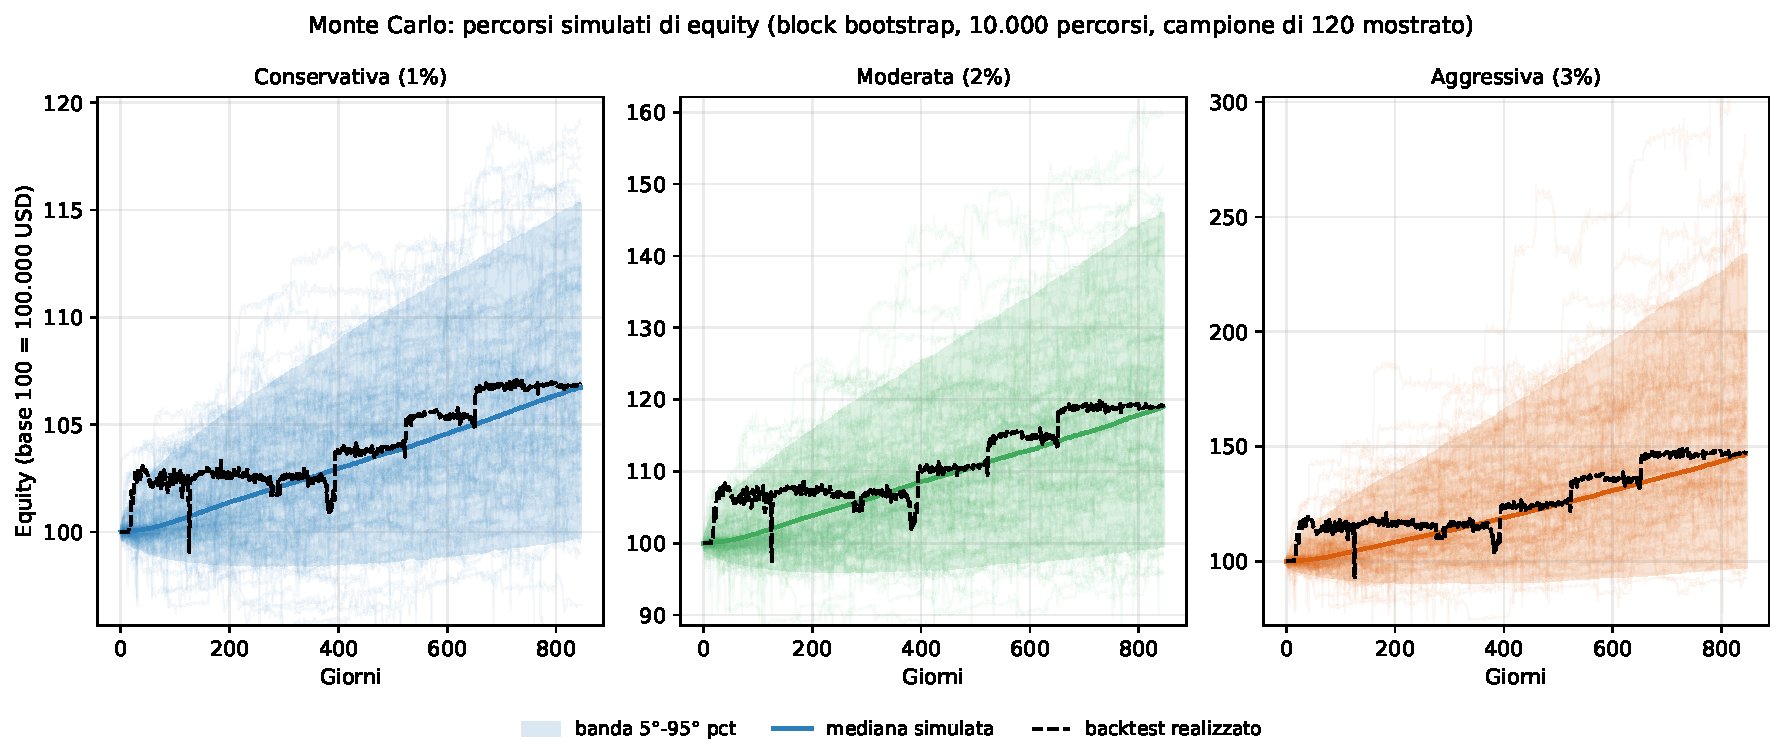
\includegraphics[width=\textwidth]{figures/fig_mc_paths.pdf}
\caption{Percorsi simulati di equity (scenario base): campione di 120
percorsi, banda 5\textsuperscript{o}--95\textsuperscript{o} percentile,
mediana simulata e curva realizzata dal backtest (tratteggiata). La curva
realizzata resta prossima alla mediana simulata in tutte le configurazioni;
la soglia di rovina (10\% dell'equity iniziale) è fuori scala, molto al di
sotto dell'intervallo mostrato.}
\label{fig:mc-paths}
\end{figure}

\chapter{Validazione statistica e cross-asset}
\label{ch:validazione}

\section{Significatività dei rendimenti}
\label{sec:val-ttest}

Il primo livello di validazione riguarda la significatività statistica dei
rendimenti. Il test $t$ sui rendimenti per trade è significativo all'1\% nel
periodo in-sample ($p = 0{,}007$), mentre nel periodo out-of-sample è
significativo soltanto al 10\% ($p = 0{,}09$): un risultato atteso, dato che
i 10 trade out-of-sample offrono una potenza statistica limitata. La
significatività in-sample, ottenuta attraversando il bear market del 2022, è
il risultato più robusto.

Poiché lo Sharpe ratio è una statistica la cui distribuzione campionaria è
sensibile alla non-normalità dei rendimenti, la sua incertezza è stata
quantificata tramite bootstrap con 10.000 ricampionamenti. Gli intervalli di
confidenza al 95\% risultano $[0{,}72;\,2{,}73]$ in-sample e
$[0{,}25;\,3{,}11]$ out-of-sample; in entrambi i casi l'intervallo non
include lo zero, e la probabilità che lo Sharpe superi l'unità è del 93\%
in-sample e del 90\% out-of-sample. La Figura~\ref{fig:bootstrap} mostra le
due distribuzioni bootstrap.

\begin{figure}[H]
\centering
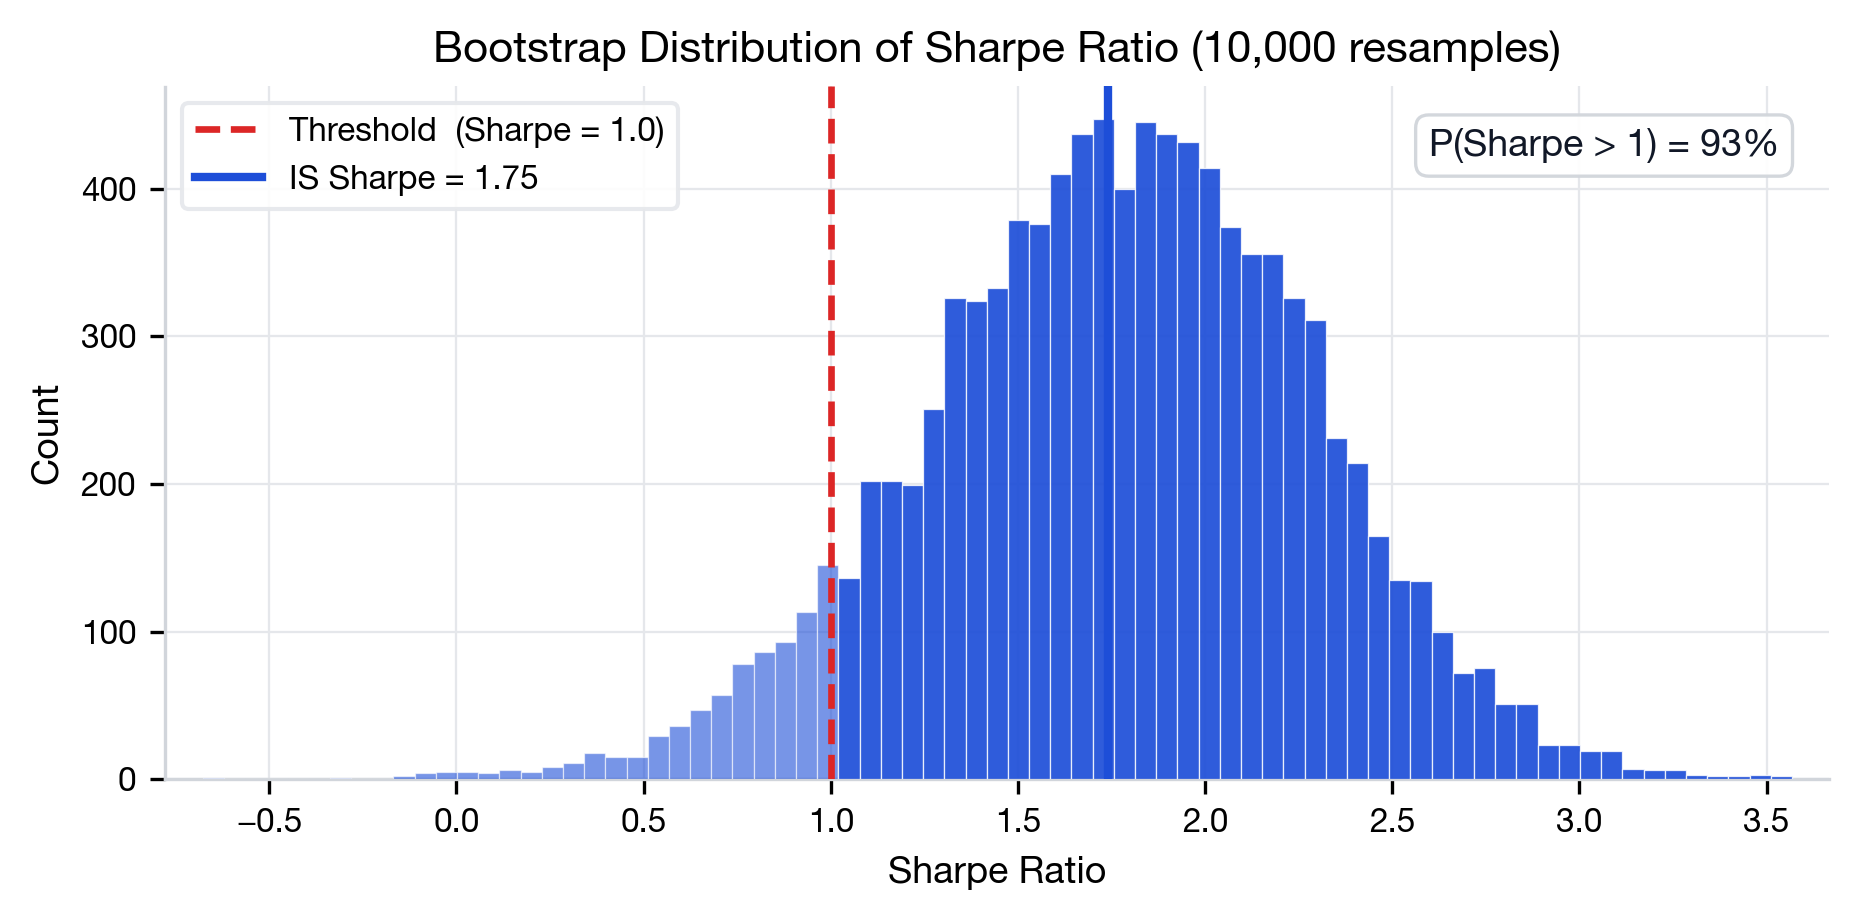
\includegraphics[width=\textwidth]{figures/fig3_bootstrap.png}
\caption{Distribuzione bootstrap dello Sharpe ratio (10.000
ricampionamenti), in-sample e out-of-sample.}
\label{fig:bootstrap}
\end{figure}

\section{Robustezza}
\label{sec:val-robustezza}

Un secondo livello di validazione verifica la robustezza del risultato a
diverse perturbazioni. La prima riguarda la dipendenza da pochi trade
eccezionali: rimuovendo i tre trade più profittevoli, lo Sharpe in-sample
scende a 1,25, restando positivo; rimuovendone cinque, scende a 0,72, ancora
positivo, mentre l'out-of-sample, ridotto a soli cinque trade, non è più
interpretabile. Il risultato in-sample non dipende quindi da un pugno di
osservazioni fortunate.

La seconda perturbazione riguarda i costi. La strategia resta profittevole
anche moltiplicando per dieci i costi di copertura correnti, un margine di
sicurezza ampio rispetto a possibili sottostime dei costi di esecuzione. La
terza riguarda i regimi: coerentemente con la natura di una strategia short
volatility, la performance è forte in regime di volatilità bassa e media e
debole in alta volatilità; sul piano della direzione del mercato, la
strategia funziona sia in fasi rialziste sia ribassiste in-sample (con win
rate del 70\% in entrambe), mentre out-of-sample è forte nelle fasi
rialziste e negativa in quelle laterali. Questo profilo è atteso e coerente
con il meccanismo, non un segno di fragilità.

L'ultima perturbazione riguarda i parametri di uscita. La
Figura~\ref{fig:sensitivity} riporta la griglia di sensibilità sui due
parametri della regola di uscita, il profit target (dal 25\% all'85\%) e la
soglia di giorni a scadenza (da 2 a 10): tutte le 30 combinazioni producono
uno Sharpe positivo (da 0,81 a 2,08) e win rate tra il 48\% e il 70\%. La
combinazione adottata (50\%, 5 giorni) non è un picco isolato della
griglia, ma un punto interno di una regione ampiamente profittevole: la
redditività della strategia non dipende da una scelta fortunata dei
parametri di uscita.

\begin{figure}[H]
\centering
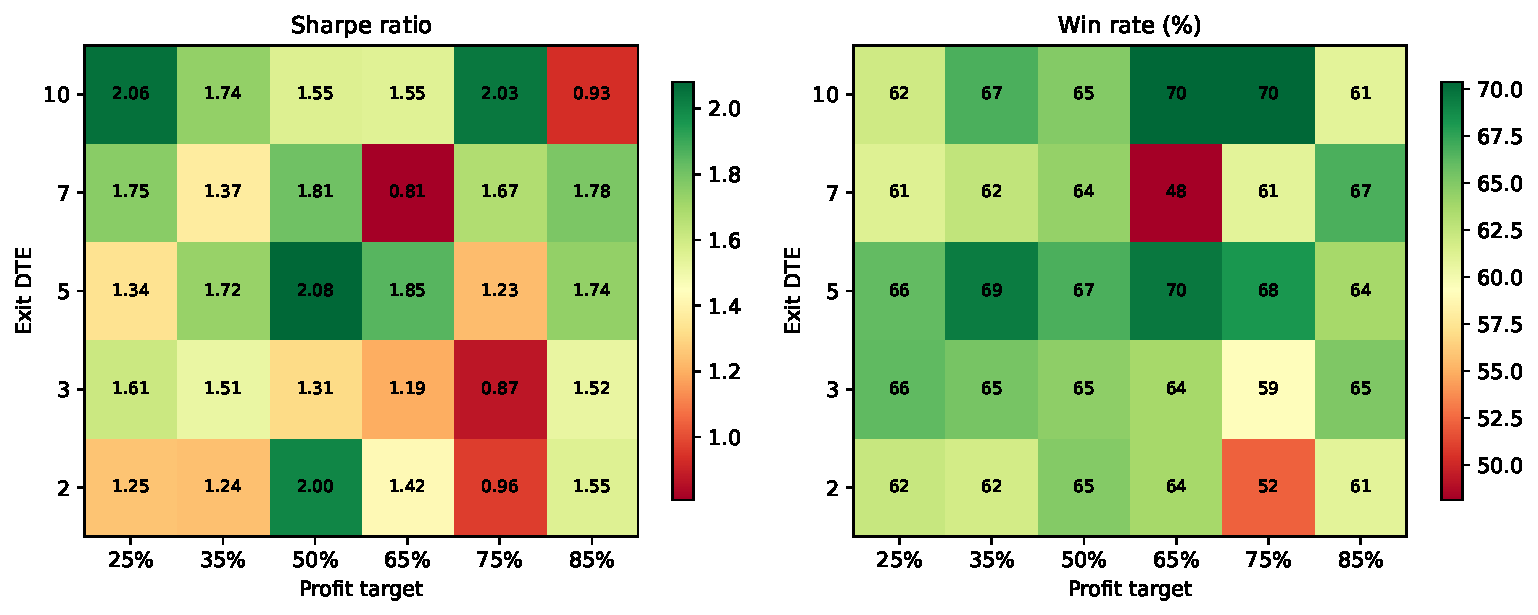
\includegraphics[width=\textwidth]{figures/fig_sensitivity.pdf}
\caption{Analisi di sensibilità sui parametri di uscita: Sharpe ratio (a
sinistra) e win rate (a destra) per ogni combinazione di profit target e
soglia di giorni a scadenza. Tutte le combinazioni sono profittevoli.}
\label{fig:sensitivity}
\end{figure}

\section{Validazione cross-asset: SPY}
\label{sec:val-spy}

Il terzo e più importante livello di validazione affronta il limite
principale del lavoro: la scarsa numerosità del campione Bitcoin. La stessa
strategia Top Vega, con gli stessi parametri e senza alcuna riottimizzazione,
è stata applicata alle opzioni SPY su quattordici anni di dati (147 trade).
L'obiettivo non è proporre una strategia sul mercato azionario, ma verificare
che il meccanismo di cattura del premio non sia un artefatto del campione
Bitcoin.

Due precisazioni metodologiche sulla trasparenza dell'esercizio. Primo,
l'audit dei costi: il primo backtest su SPY utilizzava erroneamente i costi
di Deribit (0,03\% del sottostante per le opzioni, ben superiori ai costi
azionari realistici); dopo la correzione a costi azionari appropriati
(0,65 dollari per contratto sulle opzioni, 0,01 dollari per azione sulla
copertura), il costo per trade è sceso da 140 a 9 dollari e lo Sharpe è
passato da $-0{,}89$ a $+0{,}79$. Secondo, l'audit dei dati: tre record su
9,5 milioni presentavano volatilità implicita negativa, con impatto
complessivo di $-11$ dollari, e non è stato riscontrato alcun artefatto del
tipo prezzo di uscita nullo. La Tabella~\ref{tab:cross-asset} riassume il
confronto.

\begin{table}[H]
\centering
\caption{Confronto cross-asset: la stessa strategia Top Vega su BTC e SPY,
senza riottimizzazione dei parametri.}
\label{tab:cross-asset}
\setlength{\tabcolsep}{4pt}
\begin{tabular}{lccc}
\toprule
\textbf{Metrica} & \textbf{BTC IS (3,3 anni)} & \textbf{BTC OOS (1 anno)} & \textbf{SPY (14 anni)} \\
\midrule
Trade & 35 & 10 & 147 \\
Win rate & 65,7\% & 70,0\% & 66,0\% \\
Sharpe & 1,75 & 1,52 & 0,79 \\
Return & 37,0\% & 14,3\% & 9,1\% \\
Max DD & $-7{,}0\%$ & $-4{,}7\%$ & $-2{,}3\%$ \\
IV media entry & 69\% & n.d. & 16\% \\
Costi/trade & \$100 & n.d. & \$9 \\
\bottomrule
\end{tabular}
\end{table}

Il risultato chiave emerge dalla decomposizione del profitto per trade nelle
sue due componenti, riportata nella Tabella~\ref{tab:decomposizione}.

\begin{table}[H]
\centering
\caption{Decomposizione del profitto per trade: gamba opzionaria contro
copertura. Il win rate della gamba opzionaria è identico sulle due asset
class; la differenza è interamente nell'economia della copertura.}
\label{tab:decomposizione}
\begin{tabular}{lcc}
\toprule
\textbf{Metrica} & \textbf{BTC IS} & \textbf{SPY} \\
\midrule
Win rate option-only & 82,9\% & 82,3\% \\
Win rate totale & 65,7\% & 66,0\% \\
Option PnL/trade & $+\$858$ & $+\$200$ \\
Hedge PnL/trade & $+\$298$ & $-\$129$ \\
\bottomrule
\end{tabular}
\end{table}

\begin{figure}[H]
\centering
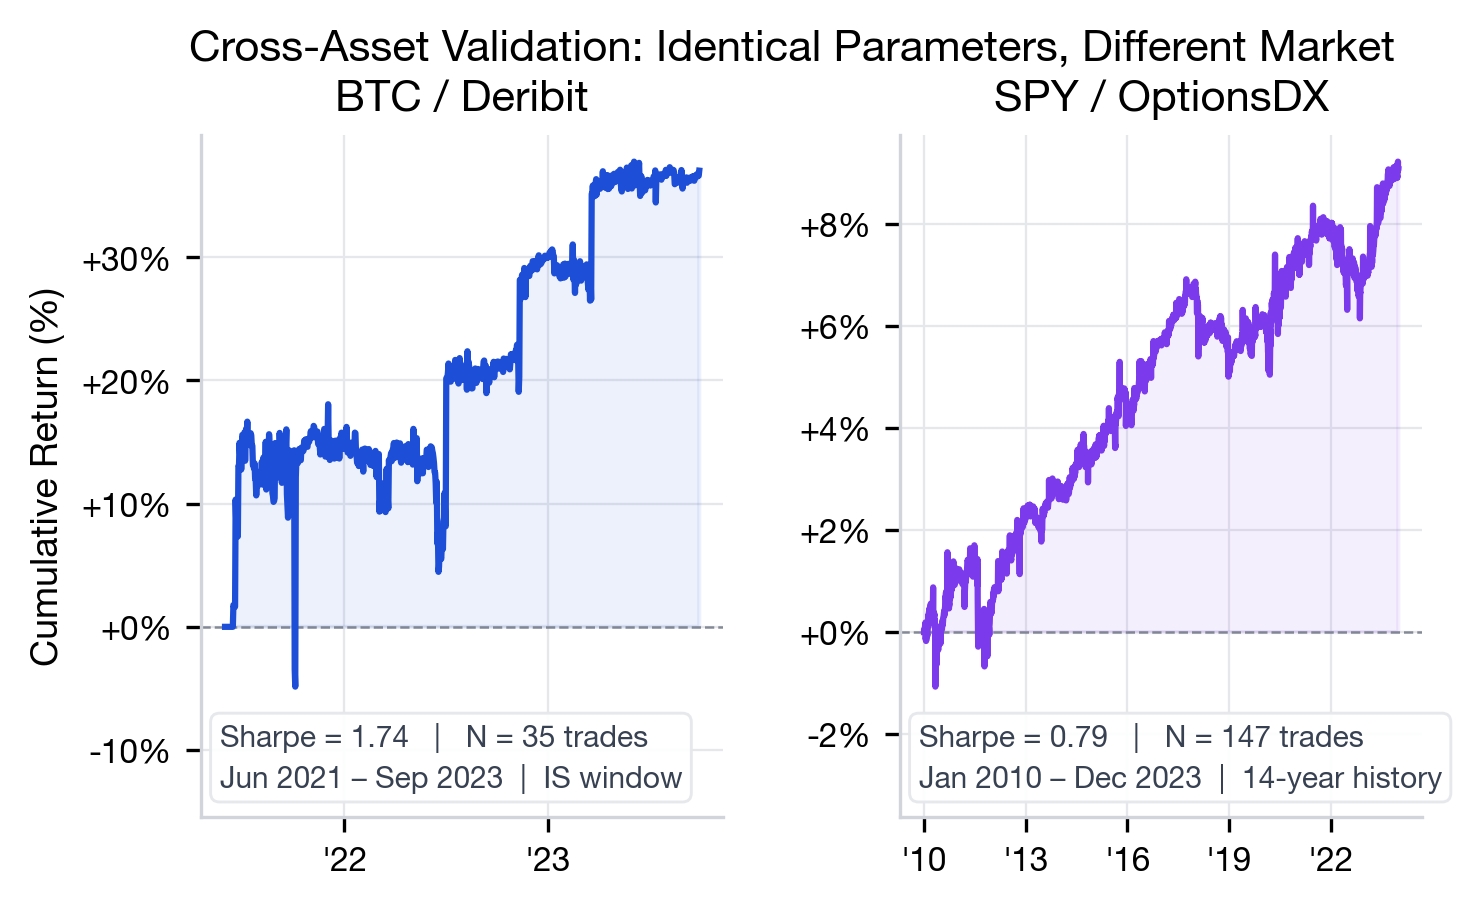
\includegraphics[width=\textwidth]{figures/fig4_crossasset.png}
\caption{Validazione cross-asset su opzioni SPY (2010--2023).}
\label{fig:crossasset}
\end{figure}

La lettura di questi risultati si articola in sei punti.

Primo, il win rate della sola gamba opzionaria è praticamente identico sulle
due asset class (82,9\% su Bitcoin, 82,3\% su SPY): il meccanismo Top Vega
cattura il premio di volatilità con la stessa efficacia su mercati molto
diversi. Questa è la prova centrale che il meccanismo non è specifico di
Bitcoin.

Secondo, la differenza di redditività risiede interamente nella copertura.
Su Bitcoin la copertura guadagna in media 298 dollari per trade, grazie
all'alta volatilità realizzata che rende profittevole il ribilanciamento
gamma; su SPY la copertura perde 129 dollari per trade, perché la volatilità
è troppo bassa e i costi di ribilanciamento superano il profitto da gamma.

Terzo, la verifica che la copertura non abbia un bias direzionale: nei soli
trade con mercato sostanzialmente piatto (rendimento del sottostante
inferiore al 2\% in valore assoluto durante il trade), la copertura su
Bitcoin genera comunque 771 dollari per trade, confermando che il profitto
proviene dal ribilanciamento gamma e non dall'esposizione direzionale; su
SPY, nelle stesse condizioni, la copertura perde 518 dollari per trade,
perché la volatilità realizzata è insufficiente a generare profitto dal
ribilanciamento.

Quarto, l'attribuzione del profitto su Bitcoin: l'81\% del profitto totale
(858 su 1.057 dollari per trade) proviene dalla vendita di opzioni, e il
19\% (298 su 1.057) dalla copertura. La strategia è dunque genuinamente una
raccolta del premio di volatilità; la copertura è un amplificatore del
rendimento su un sottostante ad alta volatilità, non la fonte principale del
profitto.

Quinto, lo Sharpe su Bitcoin è circa doppio rispetto a SPY (1,75 contro
0,79), perché il premio di volatilità su Bitcoin è strutturalmente più ampio,
data una volatilità implicita quattro volte superiore (69\% contro 16\%): il
premio incassato scala con la volatilità, mentre i costi non scalano nella
stessa misura.

Sesto, i 147 trade su quattordici anni compensano la scarsa numerosità del
campione Bitcoin. Un win rate identico (66\%) su un campione quattro volte
più ampio, e su un periodo che comprende la crisi COVID del 2020, il bear
market del 2022 e il ciclo di rialzo dei tassi della Federal Reserve,
conferma che il meccanismo è strutturale e non un artefatto.

È bene ribadire che la validazione su SPY non è presentata come una strategia
azionaria: uno Sharpe di 0,79 e un rendimento del 9,1\% su quattordici anni
non sono attraenti come proposta stand-alone. Il valore dell'esercizio è
dimostrare che il medesimo meccanismo funziona su una asset class diversa, e
che l'alpha è proporzionale al livello della volatilità implicita, il che
individua in Bitcoin, con la sua volatilità strutturalmente elevata, il
mercato in cui il premio è sufficientemente ampio da superare i costi di
copertura.

\chapter{Dall'analisi all'operatività: il paper trading}
\label{ch:paper-trading}

\section{Motivazione}
\label{sec:live-motivazione}

Un backtest, per quanto rigoroso, resta una simulazione condotta su dati
storici. Fra una strategia che funziona sui dati passati e un sistema capace
di operare autonomamente in tempo reale esiste una distanza fatta di
problemi che il backtest non pone: l'autenticazione all'exchange, il recupero
e la validazione dei dati di mercato in tempo reale, la gestione dello stato
tra un ciclo e il successivo, la traduzione di un segnale in un ordine
concreto. Per colmare questa distanza, e per verificare la replicabilità
operativa dell'intera pipeline, la strategia è stata implementata in un
sistema di paper trading che opera sulla testnet di Deribit. Questo capitolo
ne descrive l'architettura e la coerenza con il backtest.

\section{Architettura del sistema}
\label{sec:live-architettura}

Il sistema di trading in tempo reale si compone di quattro moduli, orchestrati
da un ciclo eseguito periodicamente. Il primo modulo è il client
dell'API REST di Deribit, che gestisce l'autenticazione OAuth2, il refresh
del token e le chiamate agli endpoint di mercato e di trading, con la
possibilità di operare indifferentemente su testnet o in produzione. Il
secondo modulo è lo \emph{scorer}, che replica in tempo reale la logica di
selezione Top Vega sulla catena di opzioni corrente, applicando gli stessi
filtri del backtest (opzione a vega massimo, out-of-the-money, con delta
entro la soglia e scadenza nell'intervallo ammesso). Il terzo modulo è il
\emph{position manager}, che tiene traccia delle posizioni aperte, verifica
le condizioni di uscita e persiste lo stato su file, così da sopravvivere ai
riavvii del processo. Il quarto modulo è l'\emph{order executor}, che
traduce le decisioni in ordini e che, qualora l'autenticazione fallisca,
ripiega automaticamente in modalità \emph{dry-run}, simulando l'esecuzione
senza inviare ordini reali.

Il ciclo di trading, eseguito a intervalli regolari, procede nell'ordine:
recupero e scoring della catena di opzioni, verifica delle condizioni di
uscita sulla posizione eventualmente aperta, ribilanciamento della copertura
delta, e infine, se non vi sono posizioni aperte, apertura di una nuova
posizione sull'opzione selezionata. Al termine di ogni ciclo lo stato viene
salvato.

La Figura~\ref{fig:ciclo-live} schematizza il ciclo.

\begin{figure}[H]
\centering
\begin{tikzpicture}[
  node distance=5mm and 7mm,
  box/.style={rectangle, rounded corners=2pt, draw=black!70, fill=black!4,
              minimum height=9mm, minimum width=24mm, align=center, font=\small},
  arr/.style={-{Stealth[length=2.5mm]}, thick, black!70}
]
\node[box] (fetch)   {Fetch\\option chain};
\node[box, right=of fetch] (score)   {Scoring\\Top Vega};
\node[box, right=of score] (exit)    {Verifica\\condizioni exit};
\node[box, right=of exit]  (hedge)   {Ribilanciamento\\hedge delta};
\node[box, below=9mm of hedge] (entry)   {Apertura nuova\\posizione};
\node[box, left=of entry]  (persist) {Persistenza\\stato};
\draw[arr] (fetch) -- (score);
\draw[arr] (score) -- (exit);
\draw[arr] (exit) -- (hedge);
\draw[arr] (hedge) -- (entry) node[midway, right, font=\scriptsize] {se flat};
\draw[arr] (entry) -- (persist);
\draw[arr] (persist.west) to[out=180, in=270]
  node[midway, below left, font=\scriptsize] {ciclo ogni 4 ore} (fetch.south);
\end{tikzpicture}
\caption{Il ciclo di trading del sistema live: recupero e scoring della
catena di opzioni, verifica delle uscite, ribilanciamento della copertura,
eventuale apertura di una nuova posizione e persistenza dello stato.}
\label{fig:ciclo-live}
\end{figure}

\section{Coerenza tra backtest e sistema live}
\label{sec:live-coerenza}

Il sistema live condivide con il backtest le regole, i parametri e la logica
di dimensionamento (configurazione moderata, rischio 2\% con buffer
1,5$\times$), attingendo alla stessa configurazione centralizzata. Restano
alcune differenze inevitabili tra i due contesti. Il backtest esegue con
tempistica T+1 giornaliera, mentre il sistema live opera a intervalli
infragiornalieri; il profitto della copertura, calcolato nel backtest sui
prezzi di chiusura dei futures trimestrali, nel sistema live va ricostruito
dai prezzi in tempo reale, accumulandolo tra un ciclo e il successivo.

Proprio quest'ultimo punto ha offerto una lezione operativa. Durante il
paper trading è emerso che il profitto della gamba di copertura non veniva
accumulato correttamente da un ciclo all'altro: il sistema tracciava la
posizione di copertura ma non consolidava la variazione di valore tra i
prezzi successivi del futures. Il problema è stato individuato e corretto,
introducendo un tracciamento esplicito del prezzo di copertura e
dell'accumulo del relativo profitto tra i cicli. È un esempio del tipo di
difetto che solo l'esecuzione in condizioni reali fa emergere, invisibile in
un backtest in cui l'intera storia dei prezzi è disponibile simultaneamente.

\section{Monitoraggio}
\label{sec:live-monitoraggio}

Il sistema è corredato da una dashboard di monitoraggio, mostrata nella
Figura~\ref{fig:live-dashboard}, che visualizza in tempo reale la posizione
corrente, le greche, lo stato della copertura, il profitto non realizzato e
lo storico dei trade, oltre al confronto tra la curva di equity live e
quella attesa dal backtest.

\begin{figure}[H]
\centering
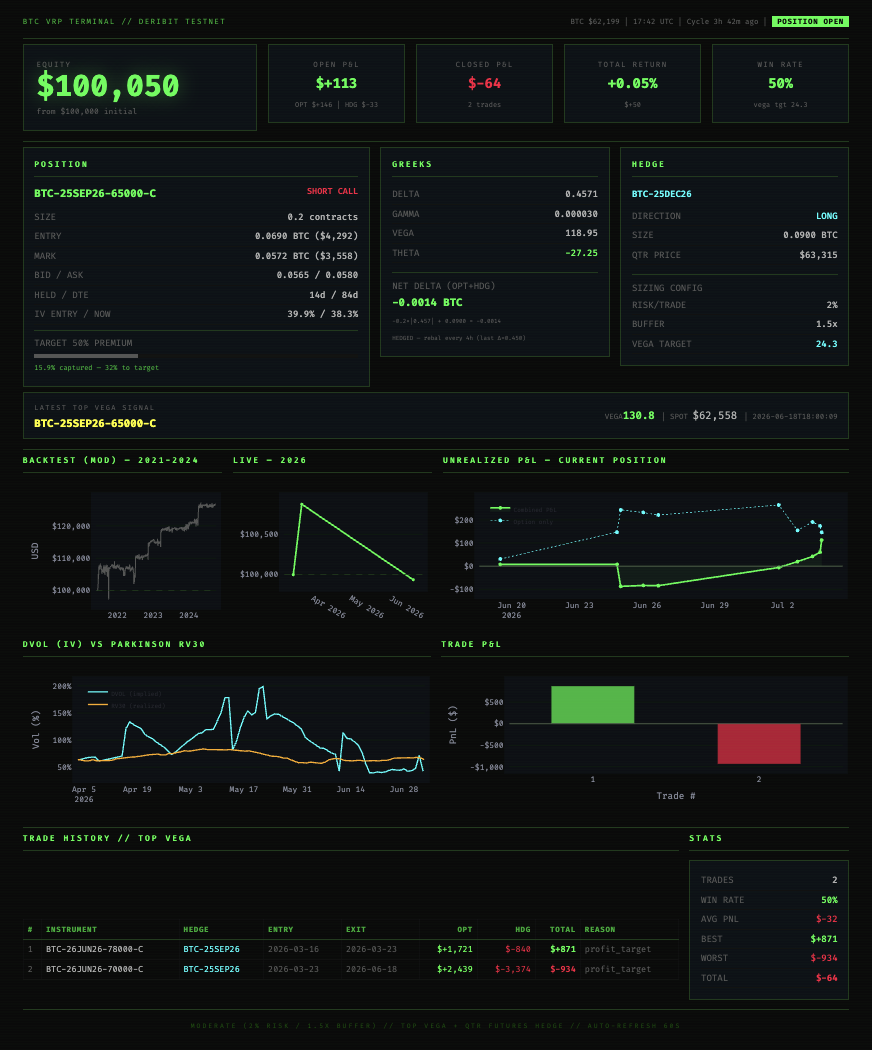
\includegraphics[width=0.8\textwidth]{figures/screen-dashboard-030702026.png}
\caption{Dashboard di monitoraggio del paper trading (testnet Deribit,
3 luglio 2026): posizione corrente e greche, stato della copertura con
futures trimestrali, segnale Top Vega più recente, confronto tra curva
di equity del backtest e curva live, profitto non realizzato della
posizione aperta e storico dei trade chiusi.}
\label{fig:live-dashboard}
\end{figure}

Alla data di questa stesura (luglio 2026) il sistema ha completato due
trade e detiene una terza posizione aperta: un campione ancora
insufficiente per qualunque valutazione statistica. I risultati
quantitativi del paper trading, con il confronto sistematico tra curva
live e curva attesa dal backtest, saranno consolidati nella versione
finale del lavoro, al termine del periodo di osservazione.

\chapter{Limitazioni e sviluppi futuri}
\label{ch:limitazioni}

Una presentazione onesta dei risultati richiede di dichiararne i limiti con
la stessa chiarezza con cui se ne espongono i pregi. Questo capitolo
raccoglie le limitazioni del lavoro, distinguendo quelle statistiche, di
esecuzione e strutturali, e indica le direzioni di ricerca che ne
discendono.

\section{Limitazioni statistiche}
\label{sec:lim-statistiche}

La limitazione più rilevante è la scarsa numerosità del campione Bitcoin: 35
trade in-sample e 10 out-of-sample. Gli intervalli di confidenza, per quanto
non includano lo zero, sono ampi, e l'analisi per regimi out-of-sample, con
così pochi trade, non è interpretabile. La validazione cross-asset su SPY
(Capitolo~\ref{ch:validazione}) è stata concepita proprio per mitigare
questo limite, ma non lo elimina sul mercato di interesse primario.

La seconda limitazione è che il periodo out-of-sample è breve e favorevole:
un mercato rialzista con volatilità in compressione gonfia verosimilmente lo
Sharpe out-of-sample rispetto a quello che ci si attenderebbe in un regime
neutro. Per questo, nella tesi, si è dato maggior peso al risultato
in-sample, che comprende invece l'episodio di stress del 2022.

La terza limitazione è l'assenza di un test formale di \emph{data snooping}
sulla strategia finale. Sebbene il percorso di ricerca
(Capitolo~\ref{ch:percorso}) documenti in modo trasparente le ipotesi
scartate, non è stato applicato un test di superiorità predittiva del tipo
di quello di \citet{hansen2005test}, che correggerebbe formalmente per la
molteplicità delle strategie considerate.

\section{Limitazioni di esecuzione}
\label{sec:lim-esecuzione}

Sul piano dell'esecuzione, la copertura delta è ribilanciata con cadenza
giornaliera, mentre Bitcoin presenta rischio di gamma e di salto anche
infragiornaliero: la copertura giornaliera lascia dunque un'esposizione
residua tra un ribilanciamento e il successivo. In secondo luogo, i prezzi
di esecuzione, pur modellati in modo conservativo (ingresso al bid, uscita
all'ask), restano idealizzati: il modello non cattura i riempimenti parziali
né lo slippage in condizioni di mercato sottili. In terzo luogo, la
protezione dal rischio di coda non è implementata, e il suo costo non è
incluso: per una strategia short volatility, l'acquisto di protezione contro
i crash è un costo reale, che una versione operativa dovrebbe internalizzare.

\section{Limitazioni strutturali}
\label{sec:lim-strutturali}

Sul piano strutturale, il vincolo di posizione singola limita la capacità
della strategia: una sola posizione alla volta su un singolo sottostante.
Come mostrato nel Capitolo~\ref{ch:percorso}, l'allentamento di questo
vincolo è stato testato e respinto per via del drawdown inaccettabile, ma
resta il fatto che la strategia ha una capacità di impiego limitata. Inoltre,
il backtest non verifica in ogni istante la sufficienza del margine Deribit:
i margini sono stati calcolati a posteriori (Capitolo~\ref{ch:money-management})
ma non integrati come vincolo dinamico nella simulazione. Infine, l'assenza
di stop loss, giustificata empiricamente, implica che la strategia richiede
la tolleranza a drawdown intraposizione significativi: non è adatta a un
investitore che non possa sostenerli.

\section{Sviluppi futuri}
\label{sec:lim-sviluppi}

Le limitazioni indicano altrettante direzioni di ricerca. Sul fronte del
segnale, il fallimento del gap RND--KDE non chiude la questione del
\emph{timing} del premio: un modello GARCH condizionale sulla misura fisica,
o un modello HAR-RV \citep{corsi2009simple} che sfrutti la memoria lunga
della volatilità realizzata, potrebbero riabilitare un segnale di timing là
dove il confronto pointwise tra densità ha fallito; anche un ensemble di
previsioni di volatilità, che in letteratura tende a battere i singoli
modelli, merita di essere esplorato.

Sul fronte del rilevamento dei regimi, con un campione più ampio
diventerebbero testabili modelli a commutazione di regime di tipo Markov,
l'uso della volatilità della volatilità come indicatore di instabilità, e
l'impiego del premio stesso come predittore dei propri rendimenti futuri,
sulla scia di \citet{bollerslev2009expected}.

Sul fronte dell'esecuzione, una versione operativa dovrebbe incorporare una
protezione dal rischio di coda calcolata dalla superficie di volatilità, una
copertura più frequente e un controllo dinamico del margine.

Infine, sul fronte delle estensioni, l'applicazione a Ethereum, il secondo
mercato di opzioni per liquidità su Deribit, è naturale una volta disponibili
dati storici adeguati. La decomposizione cross-asset del
Capitolo~\ref{ch:validazione} suggerisce inoltre una direzione controintuitiva:
poiché su SPY la gamba opzionaria è profittevole ma la copertura è un costo
netto, una struttura auto-coperta (per esempio uno strangle senza copertura
delta) potrebbe rendere la strategia profittevole anche su asset a bassa
volatilità, eliminando la componente che ne erode il rendimento.

\chapter{Conclusioni}
\label{ch:conclusioni}

Questa tesi ha affrontato una domanda operativa precisa: se il premio per il
rischio di volatilità sulle opzioni Bitcoin sia catturabile in modo
sistematico, al netto di costi di transazione realistici, attraverso una
strategia replicabile di vendita di opzioni con copertura delta. La risposta
è affermativa, e si articola in sei conclusioni.

La prima è che il premio per il rischio di volatilità su Bitcoin è reale e
catturabile in modo sistematico. La strategia Top Vega produce uno Sharpe
ratio in-sample di 1,75, statisticamente significativo all'1\%
($p = 0{,}007$), ottenuto attraversando il bear market del 2022, e al netto
di costi di transazione modellati in modo conservativo. Il premio, del resto,
è strutturalmente ampio: la volatilità implicita eccede quella realizzata nel
93\% delle giornate, con uno spread medio di 16,2 punti percentuali.

La seconda è che la strategia più semplice batte quelle più sofisticate.
La selezione dell'opzione a vega massimo, priva di parametri da stimare,
sopravvive là dove falliscono lo scoring basato sul gap tra densità, la
selezione Premium/DTE, la modalità multi-posizione, i filtri di regime e lo
stop loss. La semplicità non è un punto di partenza, ma il residuo di un
vaglio severo.

La terza è che il percorso dal complesso al semplice è esso stesso un
risultato. Documentare le cinque ipotesi scartate, ciascuna con un criterio
di rigetto quantitativo, è un contributo metodologico contro il
\emph{publication bias} che affligge la letteratura sulle strategie di
trading. In particolare, l'individuazione dell'artefatto da opzioni
illiquide con prezzo di uscita nullo, responsabile del 116\% dei profitti
apparenti di una delle strategie, è un monito di portata generale per
chiunque backtesti strategie in opzioni.

La quarta è che l'audit ha trasformato risultati apparentemente ottimi in
risultati credibili. Le distorsioni corrette nel corso del lavoro (uscite
valorizzate al bid anziché all'ask, costi assenti, opzioni illiquide con
prezzi fittizi) avrebbero prodotto una strategia illusoriamente redditizia.
Solo la loro rimozione ha reso i risultati finali difendibili.

La quinta è che il \emph{timing} del premio resta un problema aperto. Cinque
indicatori sono stati testati come possibili filtri, e nessuno ha mostrato
potere predittivo sul profitto dei singoli trade: il fattore determinante non
sono le condizioni al momento dell'ingresso, ma ciò che accade durante il
trade. Individuare un segnale di timing affidabile rimane una sfida per la
ricerca futura.

La sesta è che la validazione cross-asset conferma la natura strutturale del
meccanismo. Il win rate della sola gamba opzionaria è identico su Bitcoin e
su SPY (82\%), su un campione azionario quattro volte più ampio e su
quattordici anni che comprendono crisi ed episodi di stress. L'alpha è
proporzionale al livello della volatilità implicita: Bitcoin, con una
volatilità implicita quattro volte superiore a quella dell'indice azionario,
è il mercato in cui il premio è abbastanza ampio da superare i costi di
copertura. Il premio di volatilità è un fenomeno generale; Bitcoin è, allo
stato attuale, il luogo migliore per raccoglierlo.

Resta un'avvertenza prospettica. Il mercato delle opzioni su criptovalute è
giovane e in rapida maturazione; l'ingresso di capitale dedicato e di market
maker istituzionali potrebbe, nel tempo, comprimere il premio verso i livelli
dei mercati tradizionali. La finestra di opportunità documentata in questo
lavoro non è necessariamente permanente. La replicabilità operativa della
strategia, dimostrata dal sistema di paper trading, ne consente tuttavia il
monitoraggio continuo, così da riconoscere per tempo l'eventuale erosione del
premio che oggi rende Bitcoin un caso di studio unico.


% ════════════════════════════════════════════════════════════
\backmatter

\bibliography{bibliography}

\end{document}
